\documentclass[11pt]{cernrep}
\usepackage{graphicx,epsfig}
\bibliographystyle{lesHouches}

\usepackage{amsmath}
\usepackage{amssymb}
\usepackage{url}
\usepackage[caption=false]{subfig}


\begin{document}

%\author{Disha Bhatia$^1$, Reina Camacho$^2$, Grigorios Chachamis$^3$, Suman Chatterjee$^1$, Frederic Dreyer$^4$, Deepak Kar$^5$, Peter Loch$^6$, Ian Moult$^{7,8}$, Ben Nachman$^9$, Andreas Papaefstathiou$^{10}$, Tousik Samui$^{11}$, Andrzej Siodmok$^{12}$, Gregory Soyez$^{13}$, and Jesse Thaler$^4$}
%
%\institute{$^1$Tata Inst. of Fundamental Research, Mumbai, India
%\\$^2$Experimental Physics Department, CERN, CH-1211 Geneva 23, Switzerland
%\\$^3$Centro de Fisica Teorica y Matematicas, Madrid, Spain
%\\$^4$Center for Theoretical Physics, Massachusetts Institute of Technology, Cambridge, MA 02139, USA
%\\$^5$University of the Witwatersrand, Johannesburg, South Africa
%\\$^6$University of Arizona, Tucson, AZ 85721, USA
%\\$^7$Berkeley Center for Theoretical Physics, University of California, Berkeley, CA 94720, USA
%\\$^8$Theoretical Physics Group, Lawrence Berkeley National Laboratory, Berkeley, CA 94720, USA
%\\$^9$Physics Division, Lawrence Berkeley National Laboratory, Berkeley, CA 94720, USA
%\\$^{10}$Nikhef, Theory Group, Science Park 105, 1098 XG, Amsterdam, The Netherlands
%\\$^{11}$Indian Institute of Technology, Kanpure, India
%\\$^{12}$Theoretical Physics Department, CERN, CH-1211 Geneva 23, Switzerland
%\\$^{13}$IPhT, CEA Saclay, CNRS, Universit\'e Paris-Saclay, 91191 Gif-sur-Yvette, France}


\section{PERFORMANCE VERSUS ROBUSTNESS:  \\ TWO-PRONG SUBSTRUCTURE TAGGERS FOR THE LHC \protect\footnote{Section coordinators:  I.~Moult, B.~Nachman, G.~Soyez, J.~Thaler}$^{,}$~\protect\footnote{Contributing authors: D.~Bhatia, R.~Camacho, G.~Chachamis, S.~Chatterjee, F.~Dreyer, D.~Kar, P.~Loch, A.~Papaefstathiou, T.~Samui, A.~Siodmok}}

The ability to robustly identify, or ``tag", boosted hadronically-decaying resonances plays a central role at the LHC, both in
  searches for new physics, as well as for probing the Standard Model
  in extreme regions of phase space.
  %
  While a variety of powerful and
  theoretically well-understood tagging approaches exist, their behavior in a realistic experimental environment is complicated by a number of issues including hadronization, underlying event, pileup, and detector effects.
  %
  In this section, we perform a
  systematic study contrasting the robustness and performance of
  different theoretical approaches to designing jet substructure
  observables.
  %
  These include standard jet shape observables as well as various grooming
  strategies currently used by the LHC experiments.
  %
  We also introduce a number of new observables, based on the idea of
  ``dichroic ratios'', which are designed to simultaneously maximize both
  robustness and performance.
%
  We discuss
  the different choices used by ATLAS and CMS, and we introduce
  reliable metrics for quantifying robustness and performance for
  substructure observables.
  %
  Additionally, we study the dependence of taggers on the polarization of hadronically decaying $W$ bosons, and identify strategies to perform polarimetry using the hadronic decay products.
%  
We conclude by making recommendations for future
  tagging strategies to ensure robust procedures based on sound
  theoretical organizing principles.

%%%%%%%%%%%%%%%%%%%%%%%%%%%%%%%%%%%%%%%
\subsection{Introduction}\label{jetsub_2prong_sec:intro}
%%%%%%%%%%%%%%%%%%%%%%%%%%%%%%%%%%%%%%%

With the ever-increasing dataset from the Large Hadron Collider (LHC), we are able to probe the Standard Model and search for physics beyond the Standard Model in increasingly extreme regions of phase space.
%
Theoretically well-understood observables that are sensitive to phase space extremes are therefore playing an important role at the LHC.
%
One of the most exciting new approaches which has emerged at the LHC are tools from jet substructure, which allow for the identification of boosted hadronically-decaying particles within jets through a detailed study of their radiation patterns.
%
Techniques from jet substructure have now been widely used for Standard Model measurements \cite{Chatrchyan:2012sn,CMS:2013cda,Aad:2015cua,Aad:2015lxa,ATLAS-CONF-2015-035,Aad:2015rpa,Aad:2015hna,ATLAS-CONF-2016-002,ATLAS-CONF-2016-039,ATLAS-CONF-2016-034,CMS-PAS-TOP-16-013,CMS-PAS-HIG-16-004} as well as for searches for new physics  \cite{CMS:2011bqa,Fleischmann:2013woa,Pilot:2013bla,TheATLAScollaboration:2013qia,Chatrchyan:2012ku,CMS-PAS-B2G-14-001,CMS-PAS-B2G-14-002,Khachatryan:2015axa,Khachatryan:2015bma,Aad:2015owa,Aaboud:2016okv,Aaboud:2016trl,Aaboud:2016qgg,ATLAS-CONF-2016-055,ATLAS-CONF-2015-071,ATLAS-CONF-2015-068,CMS-PAS-EXO-16-037,CMS-PAS-EXO-16-040,Khachatryan:2016mdm,CMS-PAS-HIG-16-016,CMS-PAS-B2G-15-003,CMS-PAS-EXO-16-017}.%
\footnote{More LHC studies using jet substructure can be found at \url{https://twiki.cern.ch/twiki/bin/view/AtlasPublic} and \url{http://cms-results.web.cern.ch/cms-results/public-results/publications/}.} 

With the growing importance of jet substructure techniques, there has been a significant effort by both the theory and experimental communities to develop a more detailed understanding of the theoretical and experimental behavior of jet substructure observables.
%
On the theory side, this has been pursued through explicit calculations~\cite{Feige:2012vc,Field:2012rw,Dasgupta:2013ihk,Dasgupta:2013via,Larkoski:2014pca,Dasgupta:2015yua,Seymour:1997kj,Li:2011hy,Larkoski:2012eh,Jankowiak:2012na,Chien:2014nsa,Chien:2014zna,Isaacson:2015fra,Krohn:2012fg,Waalewijn:2012sv,Larkoski:2014tva,Procura:2014cba,Bertolini:2015pka,Bhattacherjee:2015psa,Larkoski:2015kga,Dasgupta:2015lxh,Frye:2016okc,Frye:2016aiz,Kang:2016ehg,Hornig:2016ahz,Marzani:2017mva,Marzani:2017kqd,Hoang:2017kmk,Larkoski:2017iuy,Larkoski:2017cqq}, scaling arguments~\cite{Walsh:2011fz,Larkoski:2014gra,Larkoski:2014zma}, and machine learning \cite{Cogan:2014oua,deOliveira:2015xxd,Almeida:2015jua,Baldi:2016fql,Guest:2016iqz,Conway:2016caq,Barnard:2016qma} approaches.
%
On the experimental side, there have been detailed studies of the behavior of substructure observables in data, and their interplay with experimental realities, such as detector resolution and pileup.
%
Summaries can be found in Refs.~\cite{Abdesselam:2010pt,Altheimer:2012mn,Altheimer:2013yza,Adams:2015hiv}, and Ref.~\cite{Larkoski:2017jix} provides a review of recent theoretical and machine learning developments in jet substructure. 

As a result of these efforts, there now exist a number of theoretically well-motivated jet substructure tools.
%
For tagging hadronically-decaying $W/Z/H$ bosons, which decay primarily to jets with two well-resolved prongs (also referred to as subjets), a variety of powerful two-prong taggers have been developed.
%
Modern two-prong taggers typically consist of two or three
ingredients: a groomer which removes low-energy contamination, a
two-prong finder which identifies two (or more) hard subjets, and a jet
shape observable which constrains radiation patterns in the
jet.
%
Often, the groomer and the two-prong finder are taken identical.
%
For jet shapes, it is well understood how to organize and study their
behavior using power counting \cite{Larkoski:2014gra}.
%
A variety of
different classes of observables exist, for example the energy
correlation functions \cite{Larkoski:2013eya,Moult:2016cvt,Komiske:2017aww} and $N$-subjettiness
observables \cite{Thaler:2010tr,Thaler:2011gf}, and their relation is
understood.
%
The behavior of groomers is also now well understood, and
a number of groomers with favorable experimental and theoretical properties have been introduced
\cite{Dasgupta:2013ihk,Larkoski:2014wba}.

The
theoretical understanding of the behavior of tagging observables is primarily based on perturbation theory, and it is therefore
not always clear how this translates to experimental reality, due to
the presence of hadronization, underlying event, detector effects, and
pileup.
%
Indeed, the different LHC experiments have settled on different
tagging combinations.
%
For grooming and prong finding, ATLAS using trimming \cite{Krohn:2009th} uses while CMS uses the modified
  Mass Drop Tagger (mMDT)~\cite{Butterworth:2008iy,Dasgupta:2013ihk} and its generalization, SoftDrop \cite{Larkoski:2014wba}.
  %
  For jet shape observable, ATLAS uses $D_2$ \cite{Larkoski:2014gra,Larkoski:2015kga}, while CMS uses $N$-subjettiness ratio $\tau_{2,1}$ \cite{Thaler:2010tr,Thaler:2011gf} or $N_2$ \cite{Moult:2016cvt} with DDT \cite{Dolen:2016kst}.
  %
  It is not clear whether these choices are driven by differences in the detectors, or an optimization with respect to different criteria, samples, or modeling. While detailed optimization must ultimately be performed by the experiments themselves, we believe that there is still much to be understood about the general organization and design of jet substructure observables.

In this section, we perform a comprehensive study of performance and robustness for two-prong tagging techniques.
%
To frame the study, we use a theoretical organization into different tagging strategies based on the idea of dichroic observables \cite{Salam:2016yht}, which generalize ratio observables to allow hybrid combinations of groomed and ungroomed shapes.
 %
 These contain as special instances all the familiar observables used by the experiments, as well as new observables, such as dichroic versions of the $N_2$ and $D_2$ observables.
 %
 We therefore place the ATLAS and CMS strategies as specific examples of broader classes of theoretical approaches for tagging two-prong substructure, about which we can draw general conclusions regarding robustness and performance.


The goal of this study is to highlight the interplay between performance and robustness, and assess the choices made by the different LHC experiments.
%
Here, ``performance'' refers to the tagging efficiency (for a given background rejection) in the absence of systematic uncertainties.
%
This has been the primary way to assess jet substructure observables in the past, but it does not capture the full set of considerations needed to apply jet substructure techniques in practice.
%
By contrast, ``robustness'' refers to modifications of the substructure observables as different physics aspects are added.
%
In particular, we consider robustness to non-perturbative effects, namely hadronization and underlying event, robustness to detector effects, and robustness to pileup radiation.
%
In this study, we refine the metic introduced
in Refs.~\cite{Dasgupta:2016ktv,Salam:2016yht} for quantifying
robustness.
%
We believe that this dual assessment of performance and
robustness will be useful in future studies of jet substructure
observables.
%
This allows us to study each tagging strategy in general, and the CMS
and ATLAS approaches in particular.
%
In all cases, we are able to identify observables with improved robustness and performance as compared with those currently used by the experiments.


As an additional aspect of this study, we also consider the robustness of the signal tagging efficiency to the polarization of the decaying boson.
%
We show that while jet shape observables themselves are fairly robust to polarization, groomed mass cuts are not, so that the tagging efficiency depends strongly on the polarization.
%
Furthermore, we propose that the momentum  asymmetry of the subjets is a good discriminant between longitudinal and transverse polarizations, and can be used to perform polarimetry for boosted hadronic decays. 

An outline of this study is as follows.
%
In Sec.~\ref{jetsub_2prong_sec:pres}, we define our metrics for studying robustness.
%
We discuss the key physics issues that we would like to assess robustness to, both theoretical and experimental, and describe a chain of different steps in our simulation process such that each physics issue can be isolated and studied.
%
In Sec.~\ref{jetsub_2prong_sec:obs_def}, we define all jet substructure observables that will be used throughout this study, and  provide details of our sample generation.
%
In Sec.~\ref{jetsub_2prong_sec:hybrid_ratio}, we discuss theoretical approaches to designing robust two-prong taggers.
%
We extend the approach of Ref.~\cite{Salam:2016yht} and define several new dichroic observables formed from the energy correlation functions.  
%
In Sec.~\ref{jetsub_2prong_sec:np}, we study the robustness of the observables to non-perturbative radiation both from hadronization and underlying event.
%
In Sec.~\ref{jetsub_2prong_sec:exp}, we study robustness to detector and pileup.
%
In Sec.~\ref{jetsub_2prong_sec:polar}, we study the robustness of substructure observables to the polarization of a decaying $W/Z$ boson, and introduce observables to distinguish polarized samples.
%
We summarize our results in Sec.~\ref{jetsub_2prong_sec:conc} and make a number of recommendations for future jet substructure studies.

%%%%%%%%%%%%%%%%%%%%%%%%%%%%%%%%%%%%%%%
\subsection{Quantifying Performance and Robustness}\label{jetsub_2prong_sec:pres}
%%%%%%%%%%%%%%%%%%%%%%%%%%%%%%%%%%%%%%%


The goal of this study is to study the interplay between tagging performance and robustness for two-prong taggers.
%
This requires a precise definition of the physics effects to which we are (or are not) robust, as well as a metric to quantify both performance and robustness.


Since we are able to generate pure signal and background samples, the tagging performance is straightforward to define using the signal and background efficiencies, $\epsilon_S$ and $\epsilon_B$.
%
In principle, we could evaluate the full receiver operating characteristic (ROC) curve relating $\epsilon_B$ to $\epsilon_S$.
%
For simplicity, we use the ``tagging significance'' as our metric for performance,
\begin{align}\label{eq:significance}
\epsilon=\frac{\epsilon_S}{\sqrt{\epsilon_B}}\,,
\end{align}
evaluated at a fixed signal efficiency, typically $\epsilon_S = 0.4$.

\begin{figure}[t]
\begin{center}
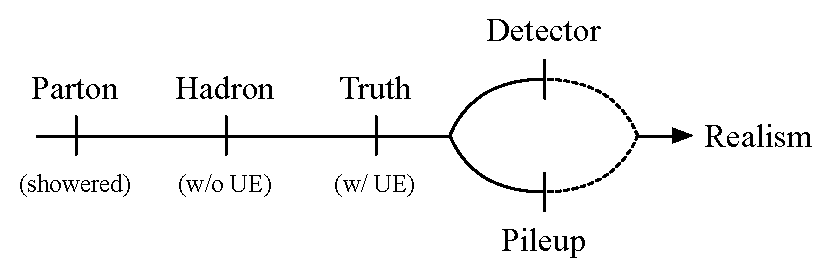
\includegraphics[width=0.75\columnwidth]{jetsub_2prong_realism_levels}
\end{center}
\caption{A summary of the different stages of physics considered in
  this study, from idealized parton-level events to fully realistic
  events including detector simulation and pileup.
  %
  This allows us to
  address robustness to physics at each stage.
  %
  Detailed definitions of
  each stage, and the physics probes used, are given in the text.
  %
   }
\label{jetsub_2prong_fig:realism}
\end{figure}

We will approach robustness by moving from an idealized partonic description to a complete detector simulation including pileup; a``realistic" scenario representative of the LHC environment.
%
This chain of realism is shown in Fig.~\ref{jetsub_2prong_fig:realism}, which illustrates the following stages:
%
\begin{itemize}
\item {\bf Parton Level}: We define the parton level result as the
  perturbative distribution for the active-active scattering (i.e.\ we
  do not include possible perturbative contributions to the underlying
  event).
  %
  While this can be defined in an analytic calculation, it is
  more difficult in the context of parton shower generators, since
  there is necessarily a cut-off that must be imposed between
  perturbative and non-perturbative physics.
  %
  Only the complete result
  is physical, and intermediate results should be interpreted with
  care.
  %
  Nevertheless, to have some measure of the impact of
  non-perturbative effects, we will define parton level as generated
  by a parton shower generator with all hadronization effects turned
  off.
  %
  We use \textsc{Pythia 8} \cite{Sjostrand:2006za,Sjostrand:2007gs} as our baseline generator, leaving a study of additional generators to future work.
%
\item {\bf Hadron Level}: We define the hadron level result as including hadronization in the shower, but not including any effects from the underlying event.
%
\item {\bf Truth Level}:  We define truth level as the hadronized result including the underlying event as implemented in an event generator.
%
Truth level therefore represents a complete hard scattering process in a hadron-hadron collider in isolation.
%
\item {\bf Detector Level}: Detector-level results are defined as truth level events passed through a detector simulation as implemented by TowerGrid.  See Sec.~\ref{jetsub_2prong_sec:det_model} for details of the detector simulation.
%
\item {\bf Pileup Level}: Due to the high pileup environment of the LHC, we include in our study also the effects of uncorrelated proton interactions. We have done this separately from detector effects to be able to isolate and study the physics effects arising from pileup and pileup subtraction schemes. Our pileup subtraction scheme is described in Sec.~\ref{jetsub_2prong_sec:pu_tech}.
%
\item {\bf Full Realism}: In the final stage of realism, we should consider events with pileup at detector
  level.
  %
  These represent, to the level that we can consider in this
  study, realistic events as seen by the experiments at the
  LHC.
  %
  Since our detector and pileup assessment is still fairly basic, we
  have left this final stage for future work.
\end{itemize}

Comparing the differences as we progress step by step through this sequence allows us to address at each stage the robustness to distinct physics issues, and we hope that our segmentation is sufficiently fine that we have a comprehensive view of robustness.
%
In particular, the different steps in the chain allow us to study robustness to the following physics: 
%
\begin{itemize}
%
\item {\bf Parton $\to$ Hadron}: Changes in the distribution from parton
  level to hadron level probe non-perturbative physics associated with
  hadronization.
  %
  For many event shapes, hadronization corrections can
  be given a field-theoretic definition in terms of a matrix element
  whose symmetry properties can be used to prove basic
  results.
  %
  Ultimately, such corrections cannot be computed
  from first principles and must be included through models, such as
  those included in parton shower generators, or through dispersive approaches or shape
  functions in analytic calculations
  \cite{Dokshitzer:1995qm,Dokshitzer:1995zt,Korchemsky:1999kt,Korchemsky:2000kp,Bosch:2004th,Hoang:2007vb,Ligeti:2008ac}.
    %
    To have the best theoretical
  control and understanding of jet substructure observables, it is
  therefore desirable that their performance is robust to the effects
  of hadronization.
  %
\item {\bf Hadron $\to$ Truth}: Changes in the distribution from hadron level to truth level probe the impact of the underlying event, namely the physics associated with interactions of the colliding protons and their remnants.
%
Such contributions are in principle both perturbative and non-perturbative.
%
They are poorly understood theoretically, and it is currently not known how to treat them systematically, or define them field theoretically.
%
It has been found empirically that the effects of underlying event are well modeled by a shape function \cite{Stewart:2014nna}, although the theoretical justification for this is not clear. Other simple theoretical models from which intuition can be gained have been proposed in Ref.~\cite{Cacciari:2009dp}.
%
The underlying event is implemented in parton shower event generators using models which are tuned to data, and we take these models as our definition of the underlying event.
%
Due to this lack of theoretical understanding, as well as the fact that radiation from the underlying event is typically not associated with the physics that we are interested in probing, it is desirable that jet substructure observables be robust to the underlying event.
%
\item {\bf Truth $\to$ Detector}: Since we are ultimately interested in using jet substructure in experiments, the behavior of the detectors plays an essential role.
%
The finite energy and spatial resolution of the detectors ultimately degrades the behavior of the observables.
%
Furthermore, the detector response must be unfolded, and is therefore difficult to compute analytically, or to include to higher accuracy. Therefore, both for performance and calculability, it is desirable that jet substructure observables are robust to detector effects.
%
\item {\bf Truth $\to$ Pileup}: Finally, due to the high pileup environment of the LHC, significant soft radiation can contaminate jet substructure observables.
%
Since this radiation is not correlated with the underlying hard scattering process, it is not associated with the physics of interest, and therefore can only act to degrade the performance.
%
Furthermore, it is difficult to model in an analytic calculation.
%
While techniques exist to mitigate pileup, as reviewed in Sec.~\ref{jetsub_2prong_sec:pu_tech}, it is desirable that the substructure observables used are as robust as possible to pileup contamination.
%
\end{itemize}
%
We will classify the first two of these as ``Theory" issues, which will be discussed in Sec.~\ref{jetsub_2prong_sec:np}, while the second two are classified as ``Experimental" issues, and will be discussed in Sec.~\ref{jetsub_2prong_sec:exp}. This decomposition is of course somewhat arbitrary, since a coherent understanding involving the complete chain is required. However, this decomposition was chosen such that the ``Theory" issues cover an idealized hadronic collision in isolation. 

\begin{figure}[t]
\begin{center}
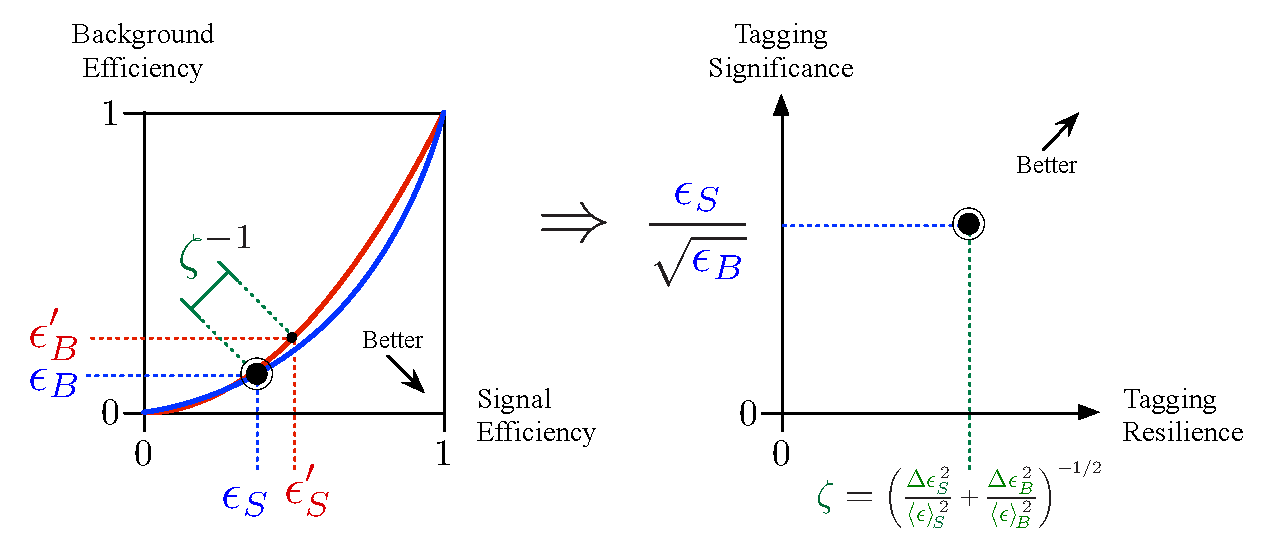
\includegraphics[width=0.9\columnwidth]{jetsub_2prong_roc_to_significance}
\end{center}
\caption{An illustration of the resilience metric $\zeta$ used throughout the text to quantify robustness. In the left panel, we illustrate graphically $\zeta$ as the change in ROC curve to a particular aspect of the underlying physics. In the right panel, we illustrate the tagging resilience vs.\ tagging performance plane which we will use to graphically illustrate our results.  A simultaneously robust and performant tagger lives in the upper right hand corner of this space}
\label{jetsub_2prong_fig:zeta_def}
\end{figure}


To compare the robustness to a
particular step in this chain for different observables, we must
introduce a metric.
%
There is of course a high degree of arbitrariness
in the definition of the metric.
%
For example, one could base the metric on the shape of the signal or background distribution.
%
Since we are ultimately interested in the performance of the observable, however, we introduce a metric which is based on the modification of the ROC curve.
%
Consider a reference stage (unprimed) and a modified stage (primed); in the case of hadronization, the reference stage would be the hadron level and the modified stage would be the parton level.
%
We first calculate the cut on the jet shape $v_{\text{cut}}$ that yields a fixed signal efficiency $\epsilon_S$ for the reference stage.
%
We then compute the reference stage background efficiency $\epsilon_B$ from that $v_{\text{cut}}$, as well as the modified stage signal and background efficiencies $\epsilon'_S$ and $\epsilon'_B$.
%
We can then defined a measure of robustness, which we refer to as resilience, $\zeta$, as
%
\begin{align}
\zeta=\left(  \frac{\Delta \epsilon_S^2}{ \langle \epsilon \rangle_S^2}  +\frac{\Delta \epsilon_B^2}{ \langle \epsilon \rangle_B^2}  \right)^{-1/2}\,,
\end{align}
%
where
%
\begin{align}
\Delta \epsilon_{S,B} & =\epsilon_{S,B}-\epsilon_{S,B}',\\
\langle \epsilon \rangle_{S,B} & = \frac{1}{2} \left(\epsilon_{S,B} + \epsilon_{S,B}'\right).
\end{align}
%
This approach gives an estimate of how much our signal and background efficiencies have changed, for a given set of cuts, when going from one stage to another.

The meaning of $\zeta$ is illustrated in Fig.~\ref{jetsub_2prong_fig:zeta_def}, where larger values of $\zeta$ correspond to improved robustness.
%
Because we anchor to a fixed $v_{\text{cut}}$, this method can even detect a uniform shift in both the signal and background distributions (even though such a shift would not change the ROC curve).
%
We therefore believe that $\zeta$ provides a reliable metric for assessing the robustness of the tagger.
%
When presenting our results, we characterize observables
in the plane of $\epsilon$ (see Eq.~\eqref{eq:significance}) versus $\zeta$, with better observables being in
the upper-right corner.
%
We find that this allows us to synthesize the
information about a large number of observables in a compact manner.
%
A
similar metric and presentation style was used in Ref.~\cite{Dasgupta:2016ktv,Salam:2016yht}
to study robustness to non-perturbative effects.
%
In addition to
showing plots of the $\epsilon$-$\zeta$ plane, we will occasionally also show the modification of the distribution
itself to provide additional insight into the robustness of the
observables.

It is important to emphasize that it is impossible to completely
characterize an optimal observable, particularly as jet substructure
observables are being used for increasingly specific
purposes.
%
We hope that the issues that we have chosen to focus on
are representative of the issues that will be important for a broad
range of applications.
%
Other aspects, such as the robustness of the substructure observable distributions to changes in the jet mass or $p_T$ cuts, which are important for certain recent applications of jet substructure \cite{Sirunyan:2017dgc,CMS-PAS-HIG-17-010,CMS-PAS-EXO-17-001,Sirunyan:2017dnz,Sirunyan:2017nvi,Aaboud:2018zba}, and have received recent interest \cite{Shimmin:2017mfk,Aguilar-Saavedra:2017rzt,Moult:2017okx}, are
beyond the scope of the current project.
However, it would be interesting to investigate them
using similar techniques.




%%%%%%%%%%%%%%%%%%%%%%%%%%%%%%%%%%%%%%%
\subsection{Observable and Sample Definitions}\label{jetsub_2prong_sec:obs_def}
%%%%%%%%%%%%%%%%%%%%%%%%%%%%%%%%%%%%%%%

In this subsection, we define all the observables that will be studied throughout this study.
%
This includes both the jet substructure shape observables and the grooming procedures.  We also present the details of our sample generation.


%%%%%%%%%%%%%%%%%%%%%%%%%%%%%%%%%%%%%%%
\subsubsection{Jet Shape Observables}\label{jetsub_2prong_sec:shape_def}
%%%%%%%%%%%%%%%%%%%%%%%%%%%%%%%%%%%%%%%

The jet shape observables that we will consider are formed from ratios of the energy correlation functions \cite{Larkoski:2013eya,Moult:2016cvt} or the $N$-subjettiness observables \cite{Thaler:2010tr,Thaler:2011gf}.
%
The $N$-subjettiness observables are defined as~\cite{Stewart:2010tn,Thaler:2010tr,Thaler:2011gf}\footnote{For this
  study, we have used the un-normalized definition of $N$-subjettiness.}
%
\begin{equation}\label{jetsub_2prong_eq:nsubdef}
  \tau_{N}^{(\beta)} =
  \sum_{1\leq i \leq n_J} p_{Ti}\min\left\{
R_{i1}^\beta,\dotsc,R_{iN}^\beta
\right\} \ .
\end{equation}
%
Here $p_{Ti}$ is the $p_T$ of particle $i$, and the sum is over all
particles in the jet.
%
The minimum is over the longitundinally-boost-invariant angle
%
\begin{align}
R_{iJ}^2 = (\phi_i-\phi_J)^2+(y_i-y_J)^2\,,
\end{align}
%
between the particle $i$ and the axis $J$.


Implicit in the definition of the $N$-subjettiness observable in
Eq.~\eqref{jetsub_2prong_eq:nsubdef} is the definition of the axes $n_i$.
%
While their
placement is unambiguous (up to power corrections) in the limit of resolved substructure, an algorithmic definition is required to
determine their behavior in the unresolved limit.
%
Two main approaches
have been used for defining the axes.
%
The first approach is to define
the $N$-subjettiness axes as the axes found using an exclusive jet
clustering algorithm. The second approach is to minimize the sum in
Eq.~\eqref{jetsub_2prong_eq:nsubdef} over possible light-like axes $n_i$.
%
In this study, we defined the axes using subjets obtained by reclustering the jet, with choices motivated by the studies in Refs.~\cite{Stewart:2015waa,Dasgupta:2015lxh}.
%
For $\beta = 1$, we recluster using the $k_t$ algorithm~\cite{Catani:1993hr} with the
  winner-take-all recombination scheme~\cite{Larkoski:2014uqa}.
%
For $\beta = 2$, we use the generalized $k_t$ algorithm~\cite{Cacciari:2011ma} with $p=1/2$.

For two-prong tagging, the relevant observable is the ratio \cite{Thaler:2010tr}
\begin{align}
\tau_{21}^{(\beta)}\equiv \frac{\tau_{2}^{(\beta)}}{\tau_{1}^{(\beta)}}\,.
\end{align}
For a jet with a well resolved two-prong structure, we have $\tau_{21}^{(\beta)}\ll 1$, while for a jet without a well resolved substructure, we have $\tau_{21}^{(\beta)}\sim 1$.
%
This observable has been extensively used at the LHC.
%
It has been calculated to LL accuracy \cite{Dasgupta:2015lxh}, and the effects of the axis definition on the perturbative behavior have been studied at NLO \cite{Larkoski:2015uaa}.

The second class of observables that we will consider are based on the energy correlation functions \cite{Larkoski:2013eya,Moult:2016cvt}.
%
Instead of correlating particles with axes, as is done for $N$-subjettiness, the idea of the energy correlation functions is to correlate $n$-tuples of particles.
%
In discussing the energy correlation functions, it is convenient to
work with dimensionless observables, written in terms of the angular
variable, $R_{ij}$ and the energy fraction variable $z_i$:
\begin{align}\label{jetsub_2prong_eq:ptratio}  
z_i\equiv\frac{p_{Ti}}{\sum_{j \in \text{jet}} p_{Tj}}\,,
\end{align}
where $p_{Ti}$ is the transverse momentum of particle $i=1,\dots,n_J$. 
%
%Tkachov \Ref{Tkachov:1995kk,Sveshnikov:1995vi,Cherzor:1997ak,Tkachov:1999py},
%
The generalized energy correlation function is defined as
\begin{equation}\label{jetsub_2prong_eq:ecf_gen}
_v e_n^{(\beta)} = \sum_{1 \leq i_1 < i_2 < \dots < i_n \leq n_J} z_{i_1} z_{i_2} \dots z_{i_n} \prod_{m = 1}^{v} \min^{(m)}_{s < t \in \{i_1, i_2 , \dots, i_n \}} \left\{ R_{st}^{\beta} \right\},
\end{equation}
where $\min^{(m)}$ denotes the $m$-th smallest element in the list.  For a jet consisting of fewer than $n$ particles, $_v e_n$ is defined to be zero.  More explicitly, the three arguments of the generalized energy correlation functions are as follows:
\begin{itemize}
\item The subscript $n$, which appears to the right of the observable, denotes the number of particles to be correlated.   
\item The subscript $v$, which appears to the left of the observable, denotes the number of pairwise angles entering the product.  By definition, we take $v \leq \binom{n}{2}$, and the minimum then isolates the product of the $v$ smallest pairwise angles.
\item The angular exponent $\beta>0$ can be used to adjust the
  weighting of the pairwise angles as for $N$-subjettiness.
\end{itemize}

In this study, we use the 2-point energy correlation function,
\begin{align}\label{jetsub_2prong_eq:explicit_twopointvar}
_1e_2^{(\beta)}&\equiv e_2^{(\beta)}=\sum_{1\leq i<j\leq n_J} z_{i}z_{j} \, R_{ij}^\beta\ ,
\end{align}
as well as the 3-point correlators,
\begin{align}\label{jetsub_2prong_eq:explicit_ecfvar}
_1e_{3}^{(\beta)}&=\sum_{1\leq i<j<k\leq n_J} z_{i}z_{j}z_{k} \min \left\{ R_{ij}^\beta\,,  R_{ik}^\beta\,, R_{jk}^\beta  \right\} \ , \nonumber \\
_2e_{3}^{(\beta)}&=\sum_{1\leq i<j<k\leq n_J} z_{i}z_{j}z_{k} \min \left\{R_{ij}^\beta R_{ik}^\beta\,, R_{ij}^\beta  R_{jk}^\beta\,,     R_{ik}^\beta R_{jk}^\beta    \right\}  \ , \nonumber \\
e_{3}^{(\beta)}\equiv ~_3e_{3}^{(\beta)}&=\sum_{1\leq i<j<k\leq n_J} z_{i}z_{j}z_{k} \, R_{ij}^\beta R_{ik}^\beta R_{jk}^\beta \,.
\end{align}
%
A number of 2-prong discriminants have been formed from the energy correlation functions~\cite{Larkoski:2013eya,Larkoski:2014gra,Larkoski:2014zma,Moult:2016cvt}.  Here, we will focus on the observables
\begin{align}
 M_2^{(\beta)} = \frac{_1e_{3}^{(\beta)}}{e_{2}^{(\beta)}}, \qquad  N_2^{(\beta)} = \frac{_2e_{3}^{(\beta)}}{(e_{2}^{(\beta)})^2}\,, \qquad  D_{2}^{(\beta)}=\frac{e_{3}^{(\beta)}}{(e_{2}^{(\beta)})^{3}}\,, 
\end{align}
each of which probes the correlations between particles within the jet in a slightly different manner.
%
For a detailed discussion, see Ref.~\cite{Moult:2016cvt}.
%
The $N_2$ and $D_2$ observables are powerful discriminants and have
been used by CMS and ATLAS, respectively.
%
The $M_2$ observable is expected to have worse performance, except in particular scenarios, but we include it since it provides an example of a remarkably robust observable.

Beyond their discrimination power, these observables have nice theoretical properties.
%
First, since they can be written as a sum over particles in the jet without reference to external axes, they are automatically ``recoil-free'' \cite{Catani:1992jc,Dokshitzer:1998kz,Banfi:2004yd,Larkoski:2013eya,Larkoski:2014uqa}.
%
Second, since they have well-defined behavior in various soft and collinear limits, they are amenable to resummed calculations;  in Ref.~\cite{Larkoski:2015kga}, $D_2$ was calculated to next-to-leading-logarithmic (NLL) accuracy in $e^+e^-$ for both signal (boosted $Z$) and background (QCD) jets, and this was extended in Refs.~\cite{Larkoski:2017iuy,Larkoski:2017cqq} to a hadron-collider environment by exploiting the simplifying properties of grooming.




%%%%%%%%%%%%%%%%%%%%%%%%%%%%%%%%%%%%%%%
\subsubsection{Grooming Techniques}\label{jetsub_2prong_sec:groom_tech}
%%%%%%%%%%%%%%%%%%%%%%%%%%%%%%%%%%%%%%%

Groomers, which remove wide-angle soft radiation and contamination from a jet, also play an important role in two-prong tagging.
%
While a variety of different grooming approaches have been defined~\cite{Butterworth:2008iy,Ellis:2009su,Ellis:2009me,Krohn:2009th,Dasgupta:2013via,Dasgupta:2013ihk}, we will focus on the mMDT/SoftDrop family, which is the most theoretically well understood, as well as trimming \cite{Krohn:2009th}, which is used by the ATLAS experiment.
%
In this subsection, we review the definition of the mMDT/SoftDrop and trimming algorithms and their parameters.

Starting from a jet identified with an IRC safe jet algorithm (such as
anti-$k_t$~\cite{Cacciari:2008gp}), the SoftDrop algorithm proceeds as follows:
%
\begin{enumerate}
%
\item Recluster the jet using the Camridge/Aachen (C/A) clustering
  algorithm~\cite{Dokshitzer:1997in,Wobisch:1998wt,Wobisch:2000dk},
  producing an angular-ordered branching history for the jet.
%
\item Step through the branching history of the reclustered jet.  At each step, check the SoftDrop condition
\begin{align}\label{jetsub_2prong_eq:sd_cut}
\frac{\min\left[ p_{Ti}, p_{Tj}  \right]}{p_{Ti}+p_{Tj}}> {z_{\rm cut}} \left(   \frac{R_{ij}}{R}\right)^\beta \,.
\end{align}
Here, ${z_{\rm cut}}$ is a parameter defining the scale below which soft radiation is removed.  If the SoftDrop condition is not satisfied, then the softer of the two branches is removed from the jet.  This process is then iterated on the harder branch.
%
\item The procedure terminates once the SoftDrop condition is satisfied.
%
\end{enumerate}
SoftDrop generalises the mMDT procedure~\cite{Dasgupta:2013ihk} and
the two are equivalent for $\beta=0$.
%
For this reason, we will often use
the two names interchangeably.
%
Any IRC-safe observable can be measured on a jet groomed with the
SoftDrop procedure, without loosing IRC safety (for $\beta > 0$).
%
The aggressivity of the SoftDrop grooming can be adjusted by
tuning the parameters ${z_{\rm cut}}$ and $\beta$.
%
Larger values of ${z_{\rm cut}}$ groom away more radiation within the jet for a fixed value of $\beta$.
%
On the other hand, as $\beta$ is increased, the grooming becomes less
severe.
%
Typical values of ${z_{\rm cut}}$ are around $0.1$, while typical
values of $\beta$ are between $0$ and $2$.

Associated with the SoftDrop algorithm, in Sec.~\ref{jetsub_2prong_sec:polar} we will study the observable $z_g$ as a means for performing polarimetry.
%
The $z_g$ observable is also referred to as the groomed momentum fraction, and is defined as
%
\begin{align}
z_g=\frac{\min\left[ p_{Ti}, p_{Tj}  \right]}{p_{Ti}+p_{Tj}}
\end{align}
%
for the first declustering that satisfies the SoftDrop criteria.
%
This observable probes the momentum sharing between the two prongs in the
jet. For $\beta \ge 0$, this observable is Sudakov safe \cite{Larkoski:2013paa,Larkoski:2015lea} on QCD
jets.

In addition to mMDT/SoftDrop, we also consider the trimming algorithm, since it is used by the ATLAS collaboration.
%
Starting from a jet of radius $R$ identified with an IRC-safe jet algorithm, trimming is defined by the following procedure:
%
\begin{enumerate}
%
\item Recluster the jet into subjets of radius $R_{\text{sub}}$.
%
\item Eliminate from the jet all particles in subjets that satisfy
  $p_{T,\text{subjet}} > z_{\text{cut}} \, p_{T,\text{jet}}$.
%
\item The trimmed jet is then defined to consist of the remaining particles.
%
\end{enumerate}
%
Trimming has been experimentally shown to be a powerful grooming algorithm, and it exhibits excellent mass resolution.
%
That said, trimming is known to suffer from non-global logarithms \cite{Dasgupta:2001sh}, and does not have a smooth spectrum as a function of the trimmed mass.
%
The trimmed mass was analytically calculated in Ref.~\cite{Dasgupta:2013ihk}.
%
The trimming parameters used by ATLAS are $R_{\text{sub}}=0.2$,  $ {z_{\rm cut}}=0.05$, and the $k_T$ algorithm is used to perform the reclustering.


%%%%%%%%%%%%%%%%%%%%%%%%%%%%%%%%%%%%%%%
\subsubsection{Parton Shower Samples}\label{jetsub_2prong_sec:samples_sub}
%%%%%%%%%%%%%%%%%%%%%%%%%%%%%%%%%%%%%%%



For our QCD background jet samples we generated $pp\to$ dijets in
\textsc{Pythia} 8.230~\cite{Sjostrand:2006za,Sjostrand:2007gs} with
the Monash13 tune~\cite{Skands:2014pea}. 
%
An explicit comparison to the \textsc{Herwig}
generator~\cite{Bahr:2008pv,Bellm:2015jjp} is left for future work.
%
Samples were generated with hadronization off (parton level), with
hadronization on but underlying event off (hadron level), and with
hadronization and underlying event on (truth level). Pileup was
included by superimposing uncorrelated minimum bias events, which are
also generated in \textsc{Pythia} 8, this time using the 4C
tune. Details of our pileup removal strategies will be described in
Sec.~\ref{jetsub_2prong_sec:pu_tech}.

For our polarized $W$ samples, we considered a $gg$ produced resonance, $X$, that decays to a pair of polarized $W$ bosons.
%
This kind of resonance decaying to longitudinally-polarized $W$s appear in warped extra-dimensional models, where the Standard Model fields propagate in the bulk.
%
On the other hand, models with graviton-like tensors with minimal couplings yield only transversely-polarized $W$ bosons.
%
They were produced with the \textsc{JHUGEN} 3.1.8~\cite{Gao:2010qx,Bolognesi:2012mm} generator, interfaced with \textsc{Pythia} 8 \cite{Sjostrand:2007gs} for parton showering including the effect of hard gluon radiation.
A resonance width of 1\% was chosen.
%
Table~\ref{jetsub_2prong_table:polarisedSamples} shows the coupling values used to generate the polarised $W$ samples (see also Ref.~\cite{Gao:2010qx} for more information). 

\begin{table}[t]
\centering
\begin{tabular}{|c|c|c|c|}
\hline
Model	&Production couplings	&Decay couplings	&Decay helicity amplitudes 	\\
\hline
$2_b^+$	& $g_1=1$		& $g_5=1$		& $f_{00}=0.98$			\\
$2_m^+$	& $g_1=1$		& $g_1=g_5=1$		& $f_{00}=0.08,f_{+-}=f_{-+}=0.46$\\	
\hline
\end{tabular}
\caption{A description of the production and decay constants used to produced the polarized $W$ samples used in this studies.}
\label{jetsub_2prong_table:polarisedSamples}
\end{table}



%%%%%%%%%%%%%%%%%%%%%%%%%%%%%%%%%%%%%%%
\subsection{Theory Approaches to Robust Ratio Observables}\label{jetsub_2prong_sec:hybrid_ratio}
%%%%%%%%%%%%%%%%%%%%%%%%%%%%%%%%%%%%%%%

The observables defined in Sec.~\ref{jetsub_2prong_sec:shape_def} are designed to
distinguish boosted bosons from QCD jets using the detailed structure
of the radiation within the jets.
%
From this perspective, it is then
immediately clear that there will be an interplay between performance
and robustness.\
%
By using a maximal amount of radiation within the jet,
the maximal information is available to identify the origin of the
jet.
%
However, an increased sensitivity to radiation also means an
increased sensitivity to contamination, both theoretically from
non-perturbative hadronization effects and underlying event, as well
as experimentally from pileup.
%
It also introduces sensitivity to the
experimental reconstruction of soft momenta in the event.
% 
On the other
hand, a tight grooming procedure, which removes radiation from within
the jet, is expected to reduce the ability to distinguish boosted
bosons from QCD jets.
%
In that context, it is interesting to see that both ATLAS and CMS
have currently adopted a tight grooming strategy.

In this subsection, we introduce a classification of different tagging strategies which will be an organizing framework for our study of robustness and performance.
%
This organization will be based on the idea of dichroic observables \cite{Salam:2016yht}, which are ratio observables constructed from combinations of groomed and ungroomed observables.
%
In Sec.~\ref{jetsub_2prong_sec:dichroic}, we review the physics of the dichroic approach for the example of the $\tau_{21}$ observable.
%
In Sec.~\ref{jetsub_2prong_sec:dichroic_new}, we generalize the dichroic construction to energy correlation function based observables and give definitions of dichroic $N_2$, $D_2$, and $M_2$ observables.
%
This allows us to have multiple concrete examples of observables for each of our general tagging strategies.
%
Then, in Sec.~\ref{jetsub_2prong_sec:dichroic_sum} we present the complete set of tagging strategies that we will consider in this work, including the different parameters we will scan within each general class.



%%%%%%%%%%%%%%%%%%%%%%%%%%%%%%%%%%%%%%%
\subsubsection{Review of the Dichroic Approach}\label{jetsub_2prong_sec:dichroic}
%%%%%%%%%%%%%%%%%%%%%%%%%%%%%%%%%%%%%%%


In Ref.~\cite{Salam:2016yht}, it was proposed that in addition to considering the standard $\tau_{21}$ observable and its groomed counterpart, one should also consider a mixed version, with a groomed denominator, and an ungroomed numerator.
%
This observable was termed ``dichroic'', since different levels of grooming are sensitive to different color structures.
%
More explicitly, Ref.~\cite{Salam:2016yht} considered the three observables:
%
\begin{align}
  \tau_{21}^{\text{large}} =\frac{\tau_2^{\text{large}}}{\tau_1^{\text{large}}}\,,
  \qquad
  \tau_{21}^{\text{small}} =\frac{\tau_2^{\text{small}}}{\tau_1^{\text{small}}}\,,
  \qquad
  \tau_{21}^{\text{dichroic}} =\frac{\tau_2^{\text{large}}}{\tau_1^{\text{small}}}\,,
\end{align}
where ``large'' refers either to the plain jet of a
lightly/loosely groomed jet and ``small'' denotes a more aggressively/tightly
groomed jet.
%
It was then argued that the dichroic combination was optimal for
performance, while also increasing the robustness to non-perturbative
contamination.
%
Here we briefly summarize the motivation for the dichroic observable.
%
Readers interested in a more detailed discussion of the dichroic approach, including perturbative calculations, are referred to Ref.~\cite{Salam:2016yht}.

\begin{figure}[t]
\begin{center}
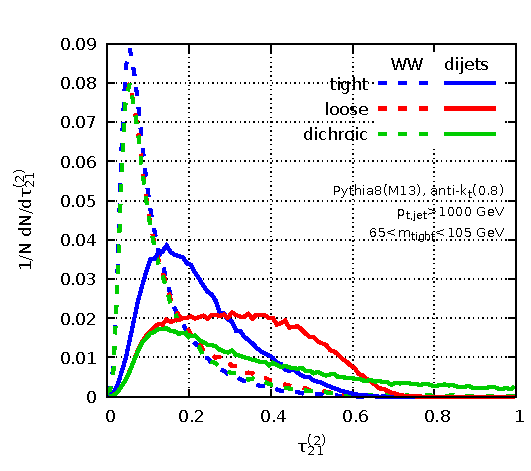
\includegraphics[width=0.5\columnwidth]{jetsub_2prong_dichroic-illust}
\end{center}
\caption{Distributions of the tight, loose, and dichroic $\tau_{21}$ observables with a cut on the mMDT/SoftDropped mass. The dichroic approach offers considerably improved performance as compared with the tight grooming, almost preserving the performance of the loose grooming at high signal purity.  Figure taken from Ref.~\cite{Salam:2016yht}.}
\label{jetsub_2prong_fig:dichroic_distribution}
\end{figure}

The benefits of the dichroic approach can simply be illustrated by
considering the distributions of the observables after aggressive
grooming (tight), moderate grooming (loose), and in the dichroic
approach.
%
This is shown in Fig.~\ref{jetsub_2prong_fig:dichroic_distribution} for the particular case of $\tau_{21}$.
%
Considerable performance is lost in going from loose to tight grooming, since the background distribution is pushed to lower values of $\tau_{21}$.
%
For the dichroic observable, by constrast, the behavior of the loose
and dichroic observables is identical at small values of $\tau_{21}$,
but for larger values of $\tau_{21}$, the dichroic distribution is
pushed to yet larger values than the loose distribution, leading to
improved performance.
%
Since the dichroic ratio observable uses a partially-groomed
observable, it is expected to be less sensitive to non-perturbative effects due to hadronization.
%
It therefore represents an interesting new class of observables to consider. 

%%%%%%%%%%%%%%%%%%%%%%%%%%%%%%%%%%%%%%%
\subsubsection{New Dichroic Observables}\label{jetsub_2prong_sec:dichroic_new}
%%%%%%%%%%%%%%%%%%%%%%%%%%%%%%%%%%%%%%%

It is almost straightforward to extend the dichroic definition from $N$-subjettiness ratios to observables formed from the energy correlation functions.
%
For $\tau_{21}$ it is immediately clear what the numerator and denominator of the observable are, however, this is initially less obvious for the energy-correlation-function-based observables that have a more complicated structure.
%
Here, we define the dichroic variants of the $M_2$, $N_2$, and $D_2$ by isolating a single factor of a mass like observable ($e_2$) as the denominator, and defining the remainder of the observable as the numerator.
%
The definitions of the dichroic variants of the $M_2$, $N_2$, and $D_2$
observables are then
\begin{align}
  M_2^{\text{dichroic}}&= \frac{( _1e_{3})^{\text{large}}  }{e_{2}^{\text{small}}}\,, \\
 N_2^{\text{dichroic}}&= \frac{\left( _{2}e_{3} / e_{2} \right)^{\text{large}} }{e_{2}^{\text{small}}}\,,\\
  D_2^{\text{dichroic}}&=\frac{\left( e_{3} / e_{2}^2 \right)^{\text{large}}}{ e_{2}^{\text{small}}}\,.
\end{align}
%
The above prescription is most easy to see for the $N_2$ observable. In the two-prong limit, the combination $ _{2}e_{3} / e_{2} $ reduces to $\tau_2$, and therefore the dichroic $N_2$ ratio behaves similarly to the dichroic $\tau_{21}$ ratio.

%%%%%%%%%%%%%%%%%%%%%%%%%%%%%%%%%%%%%%%
\subsubsection{Summary of Tagging Strategies}\label{jetsub_2prong_sec:dichroic_sum}
%%%%%%%%%%%%%%%%%%%%%%%%%%%%%%%%%%%%%%%

%%%
\begin{table}
\begin{center}
\begin{tabular}{| c | c | c |c |c|c|c |c|r| }
  \hline                       
  Observable &  Numerator & Denominator \\
  \hline
  $M_2$ &   $_{1}e_{3}$ & $ e_{2}$ \\
  $N_2$ &   $_{2}e_{3} / e_{2} $ & $ e_{2}$ \\
  $D_2$ &   $e_{3} / e_{2}^2 $ & $ e_{2}$ \\
  $\tau_{21}$ &   $\tau_2$ & $\tau_1$ \\
  \hline  
\end{tabular}
\end{center}
\caption{
Definitions of the numerators and denominators for the different jet substructure observables.
}
\label{jetsub_2prong_tab:dn}
\end{table}

%%%
\begin{table}[t!]
\begin{center}
\begin{tabular}{| c | c | c |c |c|c|c |c|c | }
  \hline                       
  Notation: $m \otimes \frac{n}{d}$ & $m$ (mass) & $n$ (numerator) & $d$ (denominator)\\
  \hline
  $p \otimes \frac{p}{p}$ & plain  &  plain & plain \\
  $\ell \otimes \frac{p}{p}$ & loose  &  plain & plain \\
  $\ell \otimes \frac{p}{\ell}$ & loose  &  plain & loose \\
  $\ell \otimes \frac{\ell}{\ell}$ & loose  &  loose & loose \\
  $t \otimes \frac{p}{p}$ & tight  &  plain & plain \\
  $t \otimes \frac{p}{\ell}$ & tight  &  plain & loose \\
  $t \otimes \frac{\ell}{\ell}$ & tight  &  loose & loose \\
  $t \otimes \frac{p}{t}$ & tight  &  plain & tight \\
  $t \otimes \frac{\ell}{t}$ & tight  &  loose & tight \\
  $t \otimes \frac{t}{t}$ & tight  &  tight & tight \\
  \hline
  $\text{trim}$ & trim &  trim & trim \\
  \hline  
\end{tabular}
\end{center}
\caption{ A summary of the different tagging strategies considered,
  including the notation, and the degree of grooming for the mass, and
  numerator and denominator of the shape observable. For simplicity,
  we have suppressed the jet radius, $R$. The definitions of plain,
  loose, tight and trim are given in the text.}
\label{jetsub_2prong_tab:tag_summary}
\end{table}

The tagging strategies we consider can be put into the general form of a (groomed) mass cut ($m$) followed by a cut on a two-prong tagging observable, which takes the form
%
\begin{align}
\mathcal{O}=\frac{\text{3-particle observable}}{\text{2-particle (mass) observable}} \equiv \frac{n}{d}\,.
\end{align}
%
The explicit numerators ($n$) and denominators ($d$) for the different observables are summarized in Tab.~\ref{jetsub_2prong_tab:dn}.

As our organizing principle for classes of  jet substructure taggers, we use the type of grooming applied to the initial mass cut, and the type of grooming applied to the numerator and denominator of the two-prong observable.
%
We use the notation 
\begin{align}
m \otimes \frac{n}{d}
\end{align}
%
to denote the grooming applied to a particular observable, where $m$, $n$, and $d$ can take the values
%
\begin{itemize}
\item plain ($p$): no grooming applied;
\item loose ($\ell$): SoftDrop with ${z_{\rm cut}}=0.05$, $\beta=2$;
\item tight ($t$): mMDT with ${z_{\rm cut}}=0.1$.
\item trim: trimming with $R_{\text{sub}}=0.2$,  $ {z_{\rm cut}}=0.05$ and the $k_T$ algorithm to perform the reclustering, as used by ATLAS.
\end{itemize}
%
In general, to have a good 2-prong tagging strategy, we want to have
\begin{align}
m \geq d \geq n\,,
\end{align}
%
where $\geq$ refers to the aggressiveness of the groomer, with $t > \ell > p$.

The complete set of configurations that we consider is given in Tab.~\ref{jetsub_2prong_tab:tag_summary}.
%
These constitute generic grooming strategies, and will be studied for each of $N_2$, $D_2$, and $\tau_{21}$.
%
They include the dichroic ratios, as well as the current ATLAS and CMS approaches as specific examples.
%
This will allow us to draw general conclusions about the performance and robustness of jet substructure taggers.


%%%
\begin{table}
\begin{center}
\begin{tabular}{| c | c | c |c |c|c|c |c|r| }
  \hline                       
  Parameter &  Values Scanned \\
  \hline
  Jet Radius $R$ &   $0.8$ \\
  Jet Shape  &   $D_2$, $N_2$, $M_2$, $\tau_{21}$  \\
  Jet Shape Angular Exponent $\beta$ &   $1$, $2$ \\
  Jet $p_T$ &   $500$ GeV, $1000$ GeV, $2000$ GeV  \\
  \hline  
\end{tabular}
\end{center}
\caption{
Jet shapes and parameters scanned for each of the different strategies proposed in Tab.~\ref{jetsub_2prong_tab:tag_summary}. 
}
\label{jetsub_2prong_tab:params}
\end{table}


While our general approach is based on studying the different classes of grooming strategies in Tab.~\ref{jetsub_2prong_tab:tag_summary}, for each of these different classes of strategies we will also scan different parameters.
%
In particular, we will scan the jet shape, jet shape angular exponent, and jet $p_T$.
%
The values scanned are summarized in Tab.~\ref{jetsub_2prong_tab:params}.
%
This allows us to understand if the conclusions drawn are associated with specific observables within a given strategy, as well as to optimize over these parameters.
%
Due to the large number of physics and detector parameters that can be
varied in our study, only a subset of plots will be presented in the
study. More specifically, we will primarily show results for the
following 3 benchmark points
%
\begin{itemize}
%
\item an {\bf ATLAS-like tagger} putting cuts on the trimmed mass and
on $D_2^{(1)}$ computed on the trimmed jet: $D_2^{(1)}\text{[trim]}$;
%
\item a {\bf CMS-like tagger} putting cuts on the mMDT mass and on
$N_2^{(1)}$ computed on the tightly-groomed jet: $N_2^{(1)}[t\otimes t/t]$;
%
\item the {\bf Les-Houches Dichroic Taggger (LHDT)} putting cuts on
  the mMDT mass and on the dichroic $D_2^{(2)}$:
  $D_2^{(2)}[t\otimes l/t]$.
%
\end{itemize}
%
To study variations, we will either fix the grooming strategy to one
of the three benchmark points and vary the jet shape, or conversely,
fix the type of jet shape to one of our benchmark points and vary the
grooming strategy.
%
A more global summary of the observables scanned, highlighting those
which we find to be most promising, will be given in
Fig.~\ref{jetsub_2prong_fig:phasespace}.

%%%%%%%%%%%%%%%%%%%%%%%%%%%%%%%%%%%%%%%
\subsection{Theory Robustness}\label{jetsub_2prong_sec:np}
%%%%%%%%%%%%%%%%%%%%%%%%%%%%%%%%%%%%%%%


In this subsection, we study robustness to hadronization and underlying event, which we categorize as ``Theory" robustness. Robustness to the detector and to pileup are treated in Sec.~\ref{jetsub_2prong_sec:exp}. 


%%%%%%%%%%%%%%%%%%%%%%%%%%%%%%%%%%%%%%%
\subsubsection{Hadronization}\label{jetsub_2prong_sec:hadr}
%%%%%%%%%%%%%%%%%%%%%%%%%%%%%%%%%%%%%%%

We begin by studying the robustness of different tagging techniques to hadronization.
%
As discussed in Sec.~\ref{jetsub_2prong_sec:pres}, this must be interpreted with some care, since the unhadronized events are not themselves physical.
%
Nevertheless, the comparison of hadronized and unhadronized distributions is the best proxy for understand the impact of hadronization short of performing an analytic calculation.
%
To ensure that our conclusions are robust, ideally we would consider parton shower generators which implement different hadronization models.
%
For example, the \textsc{Pythia} shower uses the string model \cite{Andersson:1983ia,Andersson:1998tv}, while \textsc{Herwig}$++$ uses the cluster model \cite{Webber:1983if,Marchesini:1987cf}.
%
See for example Refs.~\cite{Buckley:2011ms,Skands:2011pf,Skands:2012ts} for a more detailed discussion.
%
Due to the restricted scope of this report, here we only consider \textsc{Pythia}.
%
The effect of hadronization on two-prong substructure observables has been studied in Refs.~\cite{Larkoski:2015kga,Salam:2016yht,Larkoski:2017iuy,Larkoski:2017cqq}.

\begin{figure}
  \centering{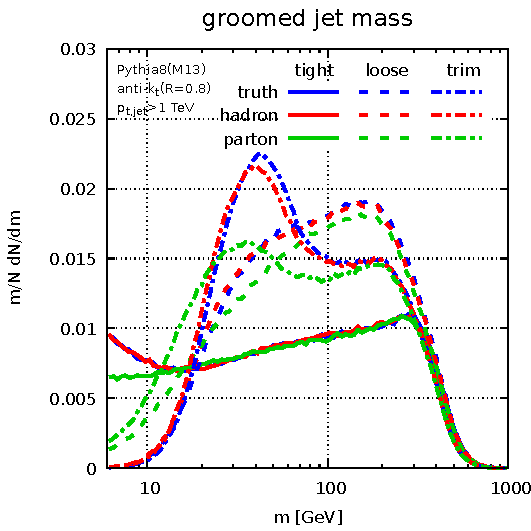
\includegraphics[width=0.4\textwidth]{jetsub_2prong_mass-distribs.pdf}}
  %
  \caption{Mass distribution after grooming for the three groomers
    considered in this paper. The distributions are shown at parton
    level, at hadron level, and at truth level (i.e.\ including both
    hadronization and the underlying event).}\label{jetsub_2prong_fig:mass-distribution}
\end{figure}

Before studying robustness under hadronization quantitatively, we begin by showing several distributions with and without hadronization.
%
This will help to introduce the different observables, as well as to give the reader a feeling for the robustness at the level of the shape of the distribution, and how this compares to our resilience measure. 

In Fig.~\ref{jetsub_2prong_fig:mass-distribution}, we show the jet-mass distribution for the three grooming strategies considered in this paper, for parton, hadron, and truth levels.
%
Although we will not focus directly on the mass distribution in this paper, it plays an important role since all of our studies will be performed with jet mass cuts.
%
Here we see two primary features.
%
First, all three groomers give rise to significantly different mass distributions.
%
This has been discussed in detail in Refs.~\cite{Dasgupta:2013ihk,Larkoski:2014wba}.
%
Second, with both tight and loose grooming, the distributions are robust to hadronization.
%
This is particularly true for tight grooming where hadronization has almost no effect, except at extremely small values of the observable.
%
On the other hand, the trimmed mass distribution is less robust to hadronization effects. 


\begin{figure}
\subfloat[]{
  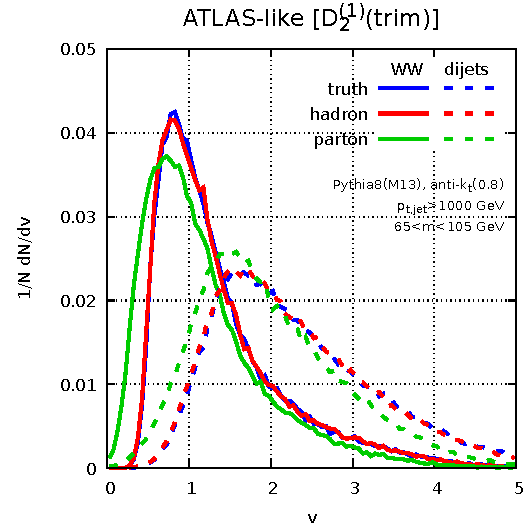
\includegraphics[width=0.32\textwidth,page=1]{jetsub_2prong_shape-distribs.pdf}
}
\subfloat[]{
  \includegraphics[width=0.32\textwidth,page=2]{jetsub_2prong_shape-distribs.pdf}
}
\subfloat[]{
  \includegraphics[width=0.32\textwidth,page=3]{jetsub_2prong_shape-distribs.pdf}
}
  \caption{Distribution of three benchmark shapes: $D_2^{(1)}$
    computed on the trimmed jet (ATLAS-like), $N_2^{(1)}$ computed on
    the tight (mMDT) jet (CMS-like), and the dichroic $D_2^{(2)}$ with numerator
    computed on the loose jet and denominator computed on the tight
    jet (LHDT). The distributions are shown at parton level, at hadron level,
    and at ``truth'' level (i.e.\ including both hadronization and the
    underlying event), for both $WW$ (solid) and dijet (dashed)
    events.}\label{jetsub_2prong_fig:shape-distribution}
\end{figure}

In Fig.~\ref{jetsub_2prong_fig:shape-distribution}, we show
distributions for our benchmark observables, namely $D_2^{(1)}$, $N_2^{(1)}$, and a dichroic version of $D_2^{(2)}$, measured on both background and signal jets.
%
In all cases, we see that hadronization has a sizable effect on the shape of the distribution, pushing it to larger values.
%
For the $D_2$ observable, hadronization is mostly isolated to small values of the observable, and at larger values reduces simply to a shift of the distribution.
%
This has been discussed in detail for the case of $D_2$ in Refs.~\cite{Larkoski:2015kga,Larkoski:2017cqq,Larkoski:2017iuy}.
%
For the $N_2$ observable, hadronization effects are larger and are significant throughout the entire distribution.
%
Indeed, when we study performance and robustness quantitatively, we will find that while $N_2$-type observables tend to be more performant, they are also less resilient to hadronization effects. 

\begin{figure}
  \centering{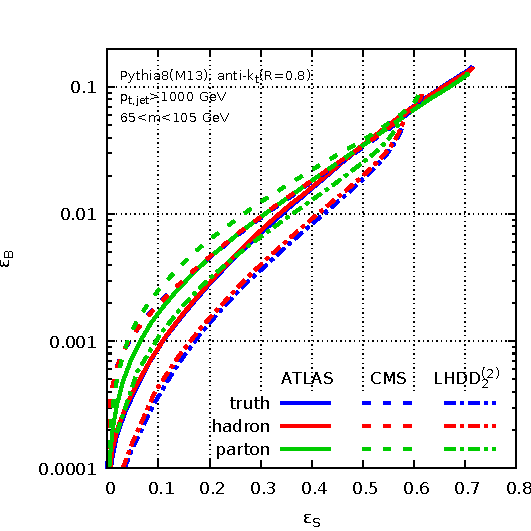
\includegraphics[width=0.4\textwidth]{jetsub_2prong_rocs.pdf}}
  %
  \caption{ROC curves corresponding to the shapes plotted on
    Fig.~\ref{jetsub_2prong_fig:shape-distribution}. The three line types correspond
    to the three benchmark points.}\label{jetsub_2prong_fig:rocs}
\end{figure}


Since the primary role of hadronization is to push the distributions to larger values at small values of the observable, the performance of the observables is typically highly sensitive to hadronization, particularly at high signal purity.
%
In Fig.~\ref{jetsub_2prong_fig:rocs} we illustrate this (lack of) robustness to hadronization at the level of the ROC curves for the different shape choices.
%
In all cases, we see that hadronization considerably improves the performance of the observables.
%
This is particularly true at high signal purity, and decreases as the signal purity is decreased.
%
Since the region of high signal purity is typically that of interest for jet substructure studies, this emphasizes the importance of understanding the robustness of observables to hadronization effects.

\begin{figure}
\begin{center}
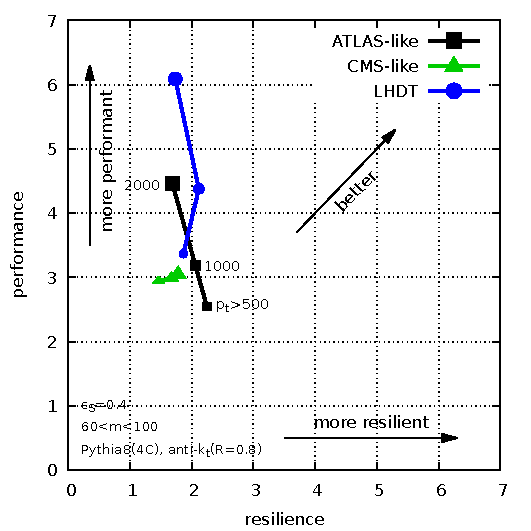
\includegraphics[width=0.4\columnwidth]{jetsub_2prong_sweep_pt}
\end{center}
\caption{An illustration of the performance-resilience plane that will be used to illustrate our results. More performant observables lie to the top, more resilient observables to the right, and better observables in the upper-right corner.}
\label{jetsub_2prong_fig:sweep_pt}
\end{figure}

Having given a feel for the modifications due to hadronization at the level of both distributions and ROC curves, we now use our performance and resilience measures to perform a quantitative study.
%
Since our visualization method allows a considerable amount of information to be condensed into a single plot, we first briefly review our presentation method with a sample plot.
%
In Fig.~\ref{jetsub_2prong_fig:sweep_pt}, we show a plot in the performance-resilience plane, in which we will display our results.
%
More performant observables appear higher on the $y$-axis (towards the top), while more robust (resilient) observables appear higher on the $x$-axis (to the right), as indicated by the arrows.
%
A performant and resilient observable will appear in the upper right corner.
%
For each observable, we also perform a scan of $p_T$, from $500-2000$ GeV, which are illustrated by the three connected points.
%
This will be the default format in which we display our results throughout the rest of this study.


\begin{figure}
\subfloat[]{
  \includegraphics[width=0.32\textwidth,page=3]{jetsub_2prong_grooming-scan.pdf}
}
\subfloat[]{
  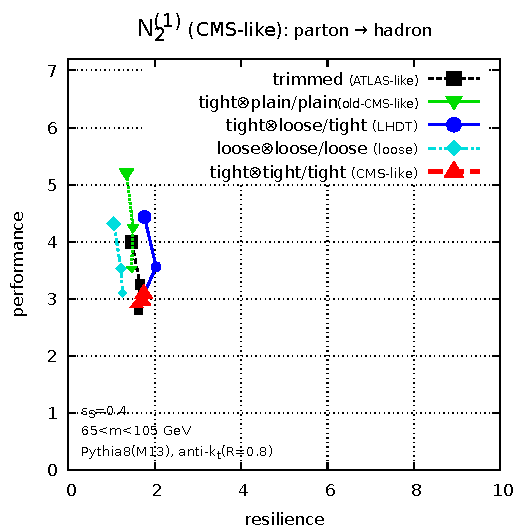
\includegraphics[width=0.32\textwidth,page=1]{jetsub_2prong_grooming-scan.pdf}
}
\subfloat[]{
  \includegraphics[width=0.32\textwidth,page=5]{jetsub_2prong_grooming-scan.pdf}
}
  \caption{Plots of the peformance-resilience plane under the addition of hadronization effects for the standard jet shape observables with different grooming strategies.}\label{jetsub_2prong_fig:grooming-hadronisation}
\end{figure}

\begin{figure}
\subfloat[]{
  \includegraphics[width=0.32\textwidth,page=5]{jetsub_2prong_shape-scan.pdf}
}
\subfloat[]{
  \includegraphics[width=0.32\textwidth,page=3]{jetsub_2prong_shape-scan.pdf}
}
\subfloat[]{
  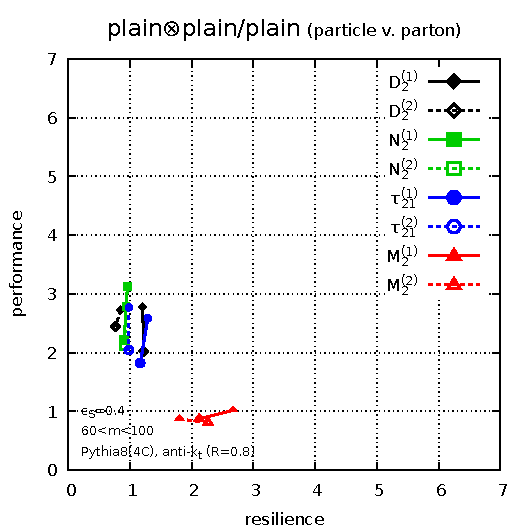
\includegraphics[width=0.32\textwidth,page=1]{jetsub_2prong_shape-scan.pdf}
}
  \caption{Plots of the peformance-resilience plane under the addition of hadronization effects for different jet shape observables, with fixed grooming strategies.}\label{jetsub_2prong_fig:shapes-hadronisation}
\end{figure}


In Figs.~\ref{jetsub_2prong_fig:grooming-hadronisation} and
\ref{jetsub_2prong_fig:shapes-hadronisation}, we show the
performance-resilience plots for the effects of hadronization for our
benchmark observables.
%
Fig.~\ref{jetsub_2prong_fig:grooming-hadronisation} shows $D_2$, $N_2$, and dichroic $D_2$ for the different grooming strategies, while in Fig.~\ref{jetsub_2prong_fig:shapes-hadronisation} we consider fixed grooming strategies in each plot, but different jet shape observables.
%
We first notice that, in almost all cases, a dichroic form of the observable can be used to improve resilience while maintaining a similar level of performance.
%
Among the shapes, we find that $D_2$ tends to be the most robust and
that $N_2$ tends to be slightly more performant, although $D_2$
becomes more performant than $N_2$ at larger $p_T$.
%
This agrees with what was seen by studying the distributions in Fig.~\ref{jetsub_2prong_fig:shape-distribution} by eye, however, we are now able to quantify this.
%
We will see that this conclusion remains true under a larger scan of observables in Sec.~\ref{jetsub_2prong_sec:exp_compare}.
%
We also notice that for almost all the observables, the trends with $p_T$ are similar.




%%%%%%%%%%%%%%%%%%%%%%%%%%%%%%%%%%%%%%%
\subsubsection{Underlying Event}\label{jetsub_2prong_sec:UE}
%%%%%%%%%%%%%%%%%%%%%%%%%%%%%%%%%%%%%%%


\begin{figure}
\subfloat[]{
  \includegraphics[width=0.32\textwidth,page=4]{jetsub_2prong_grooming-scan.pdf}
}
\subfloat[]{
  \includegraphics[width=0.32\textwidth,page=2]{jetsub_2prong_grooming-scan.pdf}
}
\subfloat[]{
  \includegraphics[width=0.32\textwidth,page=6]{jetsub_2prong_grooming-scan.pdf}
}
  \caption{Plots of the peformance-resilience plane going from hadron
    level to truth level (inclusion of underlying event) for the
    standard jet shape observables with different grooming strategies.
    %
    In this and the next figure, resilience values have been cut at
    $\zeta=10$ for easier comparison with the corresponding
    hadronisation plots,
    Figs.~\ref{jetsub_2prong_fig:grooming-hadronisation}
    and~\ref{jetsub_2prong_fig:shapes-hadronisation}.}\label{jetsub_2prong_fig:grooming-UE}
\end{figure}

\begin{figure}
\subfloat[]{
  \includegraphics[width=0.32\textwidth,page=6]{jetsub_2prong_shape-scan.pdf}
 }
\subfloat[]{
  \includegraphics[width=0.32\textwidth,page=4]{jetsub_2prong_shape-scan.pdf}
}
\subfloat[]{
  \includegraphics[width=0.32\textwidth,page=2]{jetsub_2prong_shape-scan.pdf}
}
  \caption{Plots of the peformance-resilience plane going from hadron level to truth level (inclusion of underlying event) for different jet shape observables, with fixed grooming strategies.}\label{jetsub_2prong_fig:shapes-UE}
\end{figure}


We can now repeat the same exercise performed for hadronization to study the robustness to underlying event.
%
The results in the performance-resilience plane are shown in Figs.~\ref{jetsub_2prong_fig:grooming-UE} and \ref{jetsub_2prong_fig:shapes-UE}.
%
These are identical to Figs.~\ref{jetsub_2prong_fig:grooming-hadronisation} and \ref{jetsub_2prong_fig:shapes-hadronisation} but measure the robustness to underlying event instead of hadronization.
%
The first thing that is clear from comparing Figs.~\ref{jetsub_2prong_fig:grooming-hadronisation} and \ref{jetsub_2prong_fig:shapes-hadronisation} with  Figs.~\ref{jetsub_2prong_fig:grooming-UE} and \ref{jetsub_2prong_fig:shapes-UE} is that with modern grooming techniques, we are comparatively much less sensitive to underlying event than to hadronization effects.
%
With the exception of the tight$\otimes$plain/plain grooming strategy
(which indeed does not groom the observable), all the standard
observables are robust to underlying event for all the different
grooming strategies. Similarly, all the different jet shape
observables in this study are also robust to Underlying Event
effects. The dichroid $D_2^{(2)}$ observable
(Figs.~\ref{jetsub_2prong_fig:grooming-hadronisation}c
and~\ref{jetsub_2prong_fig:grooming-UE}c) shows a smaller resilience
against the Underlying Event although it remains much larger than the
corresponding resilience to hadronisation effects.
%
We believe that this should be viewed as a success of modern grooming tools.
%
We also believe that it is desirable, since underlying event effects are much less under theoretical control than hadronization effects. 




%%%%%%%%%%%%%%%%%%%%%%%%%%%%%%%%%%%%%
\subsubsection{Towards Improved Performance and Robustness for ATLAS and CMS}\label{jetsub_2prong_sec:exp_compare}
%%%%%%%%%%%%%%%%%%%%%%%%%%%%%%%%%%%%%


\begin{figure}
\begin{center}
\subfloat[]{\label{jetsub_2prong_fig:unsoftdropped}
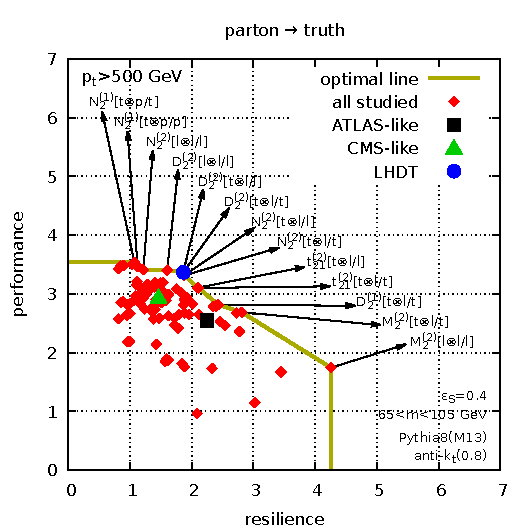
\includegraphics[width=7cm]{jetsub_2prong_optimal_pt_500}    
}\qquad
\subfloat[]{\label{jetsub_2prong_fig:softdropped}
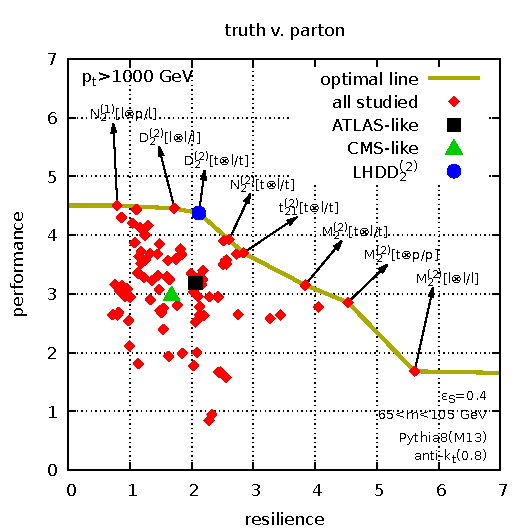
\includegraphics[width=7cm]{jetsub_2prong_optimal_pt_1000}
}
\end{center}
\caption{The performance-resilience plane for the different observables scanned in our study at (a) $500$ GeV and (b) $1000$ GeV. The ATLAS- and CMS-like observables are marked in black and green, respectively. In both cases, more robust, and more performant observables can be selected, and a number of such observables are marked.
}
\label{jetsub_2prong_fig:phasespace}
\end{figure}

The strategies used by ATLAS and CMS, namely trimmed $D_2$ \cite{Larkoski:2015kga,Larkoski:2014gra} and SoftDropped $N_2$ \cite{Moult:2016cvt} with DDT \cite{Dolen:2016kst} are specific examples of the broader approaches to two-prong tagging discussed above, and therefore our study allows us to gain insight into the different tagging strategies used by the collaborations,\footnote{And perhaps even into the sociology of the different experiments! However, such conclusions should be taken with a grain of salt.} as well as to suggest improved observables.

An overall scan of all the observables used in this study in the performance-resilience plane is shown in Fig.~\ref{jetsub_2prong_fig:phasespace}.
%
The current CMS and ATLAS observables are highlighted with the black and green markers, respectively. We can draw two interesting conclusions from this plot.
%
First, for $p_T> 500$ GeV, it appears as though ATLAS is using a more robust, but less performant observable, while CMS is using a more performant, but less robust observable.
%
This must be caveated by the fact that we have not performed a full detector study, though it is suggestive.
%
Second, we can choose from the observables considered in our study observables that are simultaneously more performant, and more resilient than those that are currently being used.
%
At $500$ GeV the gains in performance are fairly minimal, but at $1000$ GeV, it seems that there are considerable gains in performance and robustness to be made.
%
The names of a large variety of those observables which lie on the upper boundary of the performance-resilience space are marked in the figure. 


Looking more closely at the observables along this upper boundary, we see that there is in fact considerable structure, and a number of general lessons can be learned.
%
First, as we move along this boundary from least resilient to most resilient, we transition from $N_2^{(1,2)}$ observables which are the most performant, but less robust, through $D_2^{(2)}$, to $M_2^{(2)}$, which is more robust, but less performant.
%
This was also clearly observed in the distributions of Fig.~\ref{jetsub_2prong_fig:shape-distribution}.
%
We believe that this is due to the fact that $N_2$ has a hard phase space boundary, and therefore non-perturbative effects are not isolated at small values of the observable, although it would be interesting to understand this behavior in more detail. 

A second pattern that is observed is that, in almost all cases, dichroic variants of the observables of the form $t\otimes \frac{p}{t}$ or $t\otimes\frac{\ell}{t}$ exhibit improved performance without significant loss in resilience.
%
We believe that it is worthwhile for the experiments to consider some of the dichroic observables that were newly introduced in Sec.~\ref{jetsub_2prong_sec:dichroic_new} with simultaneous performance and resilience in mind.
%
We have highlighted in Fig.~\ref{jetsub_2prong_fig:phasespace} that a whole interesting phase space of such observables exist, which map out the performance-resilience plane.
%
Different observables could be chosen depending on the particular
needs of a given study.
%
Note finally, that the above study has been carried using a specific
choices of grooming strategies (loose and tight). There is therefore a
potential additional gain that can be achieved by studying alternative
(more or less aggressive) options.


%%%%%%%%%%%%%%%%%%%%%%%%%%%%%%%%%%%%%%%
\subsection{Experimental Robustness}\label{jetsub_2prong_sec:exp}
%%%%%%%%%%%%%%%%%%%%%%%%%%%%%%%%%%%%%%%

Having discussed robustness to theoretical issues, we now continue through our chain of realism of Fig.~\ref{jetsub_2prong_fig:realism} and consider robustness to detector effects.
%
In Sec.~\ref{jetsub_2prong_sec:det_model} we describe our detector model.
%
In Sec.~\ref{jetsub_2prong_sec:pu_tech} we describe pileup removal.
%
In Sec.~\ref{jetsub_2prong_sec:detector_robust} we study the robustness of jet mass to detector effects.
%
A more comprehensive study is left to a dedicated publication.

%%%%%%%%%%%%%%%%%%%%%%%%%%%%%%%%%%%%%%%
\subsubsection{Detector Models}\label{jetsub_2prong_sec:det_model}
%%%%%%%%%%%%%%%%%%%%%%%%%%%%%%%%%%%%%%%





\begin{table}\centering
\renewcommand{\arraystretch}{1.25}
\begin{tabular}{|l|c|c|c|r@{\ =\ }l|}
\hline
Signal  & \multicolumn{5}{c|}{Model parameters}    \\ \cline{2-6}                      
        & Coverage
        & \ensuremath{p_{\text{T}}^{\text{min}}}
        & \ensuremath{p_{\text{T}}^{\text{max}}} 
        & \multicolumn{2}{c|}{Resolution function parameters} \\
\hline
\multicolumn{6}{|c|}{\textbf{Configuration A} ($R_{\text{calo}} = 1150$ mm, $B_{\text{solenoid}} = 2$ T)} \\
\hline
Towers     & $|\eta| < 2.5$ & 500 MeV &  10 TeV   & \ensuremath{a_{\text{calo}}} & $10\%\times\sqrt{\text{GeV}}$                  \\ 
(EM)       &                &         &           & \ensuremath{b_{\text{calo}}} & 0                                        \\
           &                &         &           & \ensuremath{c_{\text{calo}}} & 0.7\%                                    \\
Towers     & $|\eta| < 4.9$ & 500 MeV &  10 TeV   & \ensuremath{a_{\text{calo}}} & $50\%\times\sqrt{\text{GeV}}$                  \\
(HAD)      &                &         &           & \ensuremath{b_{\text{calo}}} & 0                                        \\
           &                &         &           & \ensuremath{c_{\text{calo}}} & 3\%                                      \\
\hline 
\multicolumn{6}{|c|}{\textbf{Configuration C} ($R_{\text{calo}} = 1290$ mm, $B_{\text{solenoid}} = 4$ T)} \\
\hline
Towers     & $|\eta| < 2.5$ & 500 MeV &  10 TeV   & \ensuremath{a_{\text{calo}}} & $3\%\times\sqrt{\text{GeV}}$                   \\
(EM)       &                &         &           & \ensuremath{b_{\text{calo}}} & 0                                        \\
           &                &         &           & \ensuremath{c_{\text{calo}}} & 0.5\%                                    \\
Towers     & $|\eta| < 4.9$ & 500 MeV &  10 TeV   & \ensuremath{a_{\text{calo}}} & $100\%\times\sqrt{\text{GeV}}$                 \\
(HAD)      &                &         &           & \ensuremath{b_{\text{calo}}} & 0                                        \\
           &                &         &           & \ensuremath{c_{\text{calo}}} & 5\%                                      \\
Tracks     & $|\eta| < 2.5$ &  1 GeV  &  300 GeV  & \ensuremath{a_{\text{track}}}  & $0.015\%\times\text{GeV}^{-1}$                  \\
           &                &         &           & \ensuremath{c_{\text{track}}} & 0.5\%                                     \\
\hline
\end{tabular}
\caption{Principal properties and smearing parameters of the detector model configurations A and C. Electromagnetic (EM) towers have a tower size of $\Delta\eta\times\Delta\phi = 0.025\times0.025$, while hadronic (HAD) towers have $\Delta\eta\times\Delta\phi = 0.1\times0.1$. Tracks are not modeled in configuration A, while configuration C models both tracks and calorimeter signals to simulate the effect of a particle flow algorithm. The resolution function parameters \ensuremath{a_{\text{calo}}}, \ensuremath{b_{\text{calo}}}{}, and \ensuremath{c_{\text{calo}}}{} are used together with the resolution function in Eq.~\eqref{jetsub_2prong_eq:caloreso} to determine the width of the Gaussian energy smearing.
Similarly, \ensuremath{a_{\text{track}}}{} and \ensuremath{c_{\text{track}}}{} are used in Eq.~\eqref{jetsub_2prong_eq:trkreso} to determine the width of the track-\ensuremath{p_{\text{T}}}{} resolution smearing.}
\label{jetsub_2prong_tab:detmodel}
\end{table}





\begin{figure}
\begin{center}
\subfloat[]{
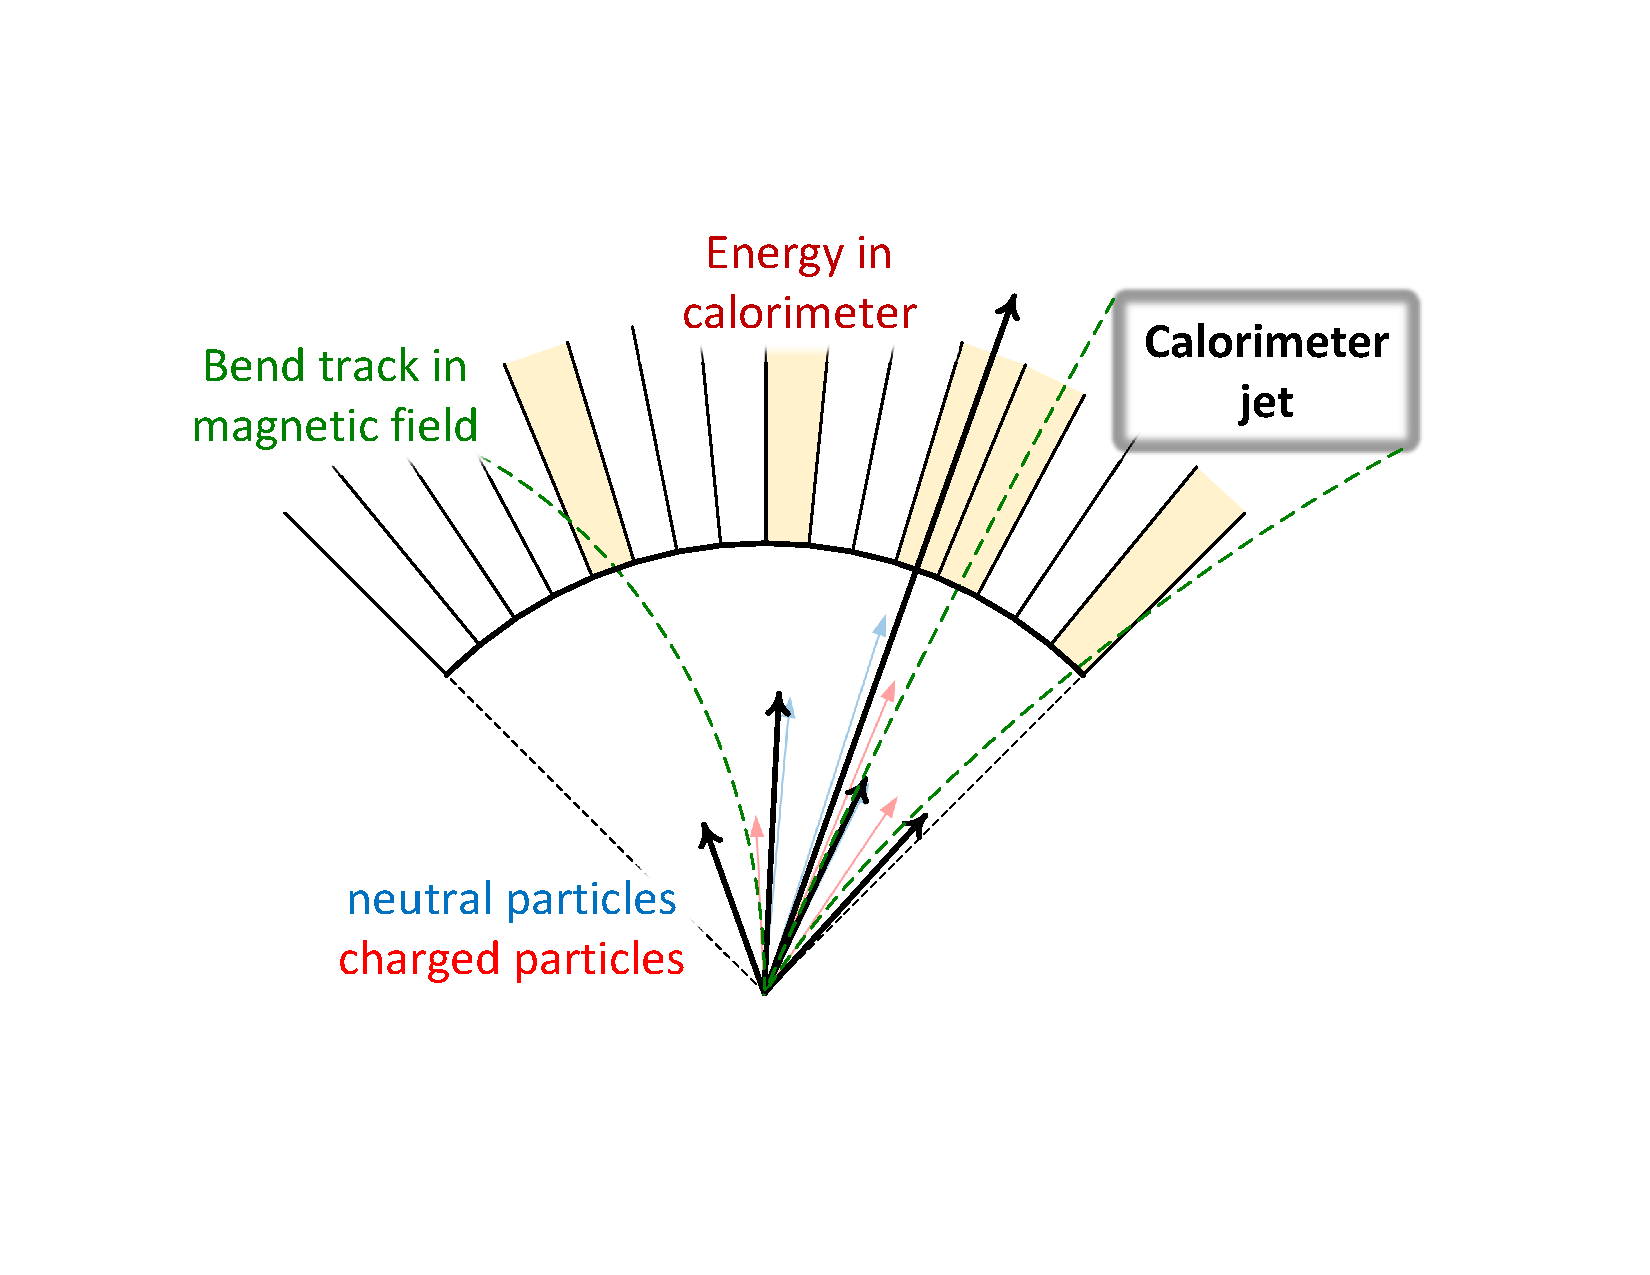
\includegraphics[width=0.48\columnwidth]{jetsub_2prong_jets_in_atlas}
}
\subfloat[]{
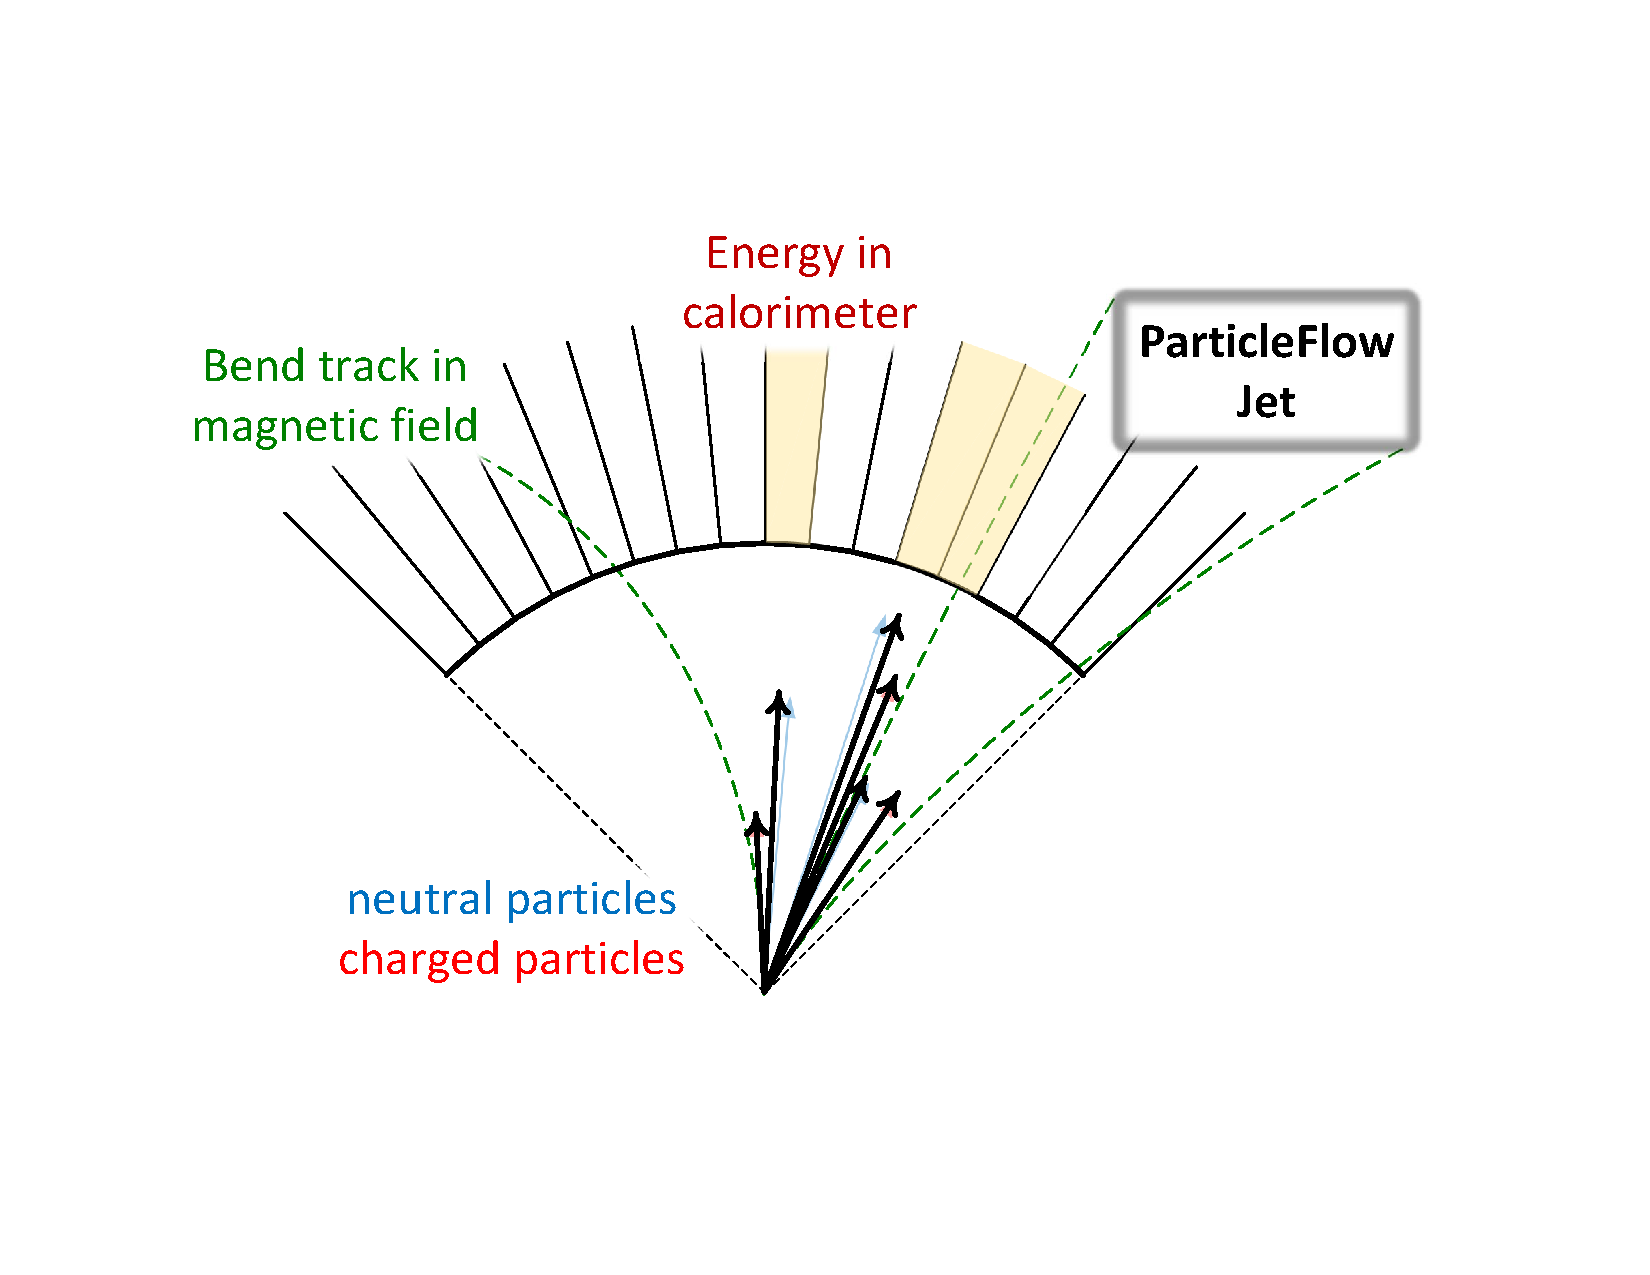
\includegraphics[width=0.48\columnwidth]{jetsub_2prong_jets_in_cms}
}
\end{center}
\caption{An illustration of the basic jet features for the configuration A (ATLAS-like, calorimeter only) and configuration C (CMS-like, particle flow using tracks and calorimeter) detector signal models. The solid black arrows indicate the jet composition from representations of neutral (pale blue) and charged (pale red) particles by calorimeter towers or reconstructed tracks. The green dashed curves show charged particle tracks bend in the magnetic field. Both illustrations show the same truth-level jet.}
\label{jetsub_2prong_fig:detmodel}
\end{figure}


%%%%% PL Jan-24-2018
The detector response is modeled by subjecting the particle-level objects\footnote{Those are stable particles produced by the generator that potentially reach a detector.  This principally requires a particle lifetime $\tau$ in the laboratory frame given by $c\tau > 10$ mm.}
to a simple acceptance and smearing model representing tracking detectors as well as calorimeters.
%
Basic detector feature descriptors are considered together with response features and signal reconstruction strategies similar to the ATLAS and CMS experiments at the LHC.
%
The respective model configurations are A (ATLAS{\emph{-like}} \cite{PERF-2007-01}) and C (CMS\emph{-like} \cite{CMS-TDR-08-001}).
%
Effects from particles showering in calorimeters are not modeled. 

Both configurations feature cylindrical detectors around the collision vertex with full azimuthal coverage $-\pi < \phi < \pi$.
The detector modeling produces a final state represented by a list of \emph{pseudoparticles} which are proxies for detector signals generated by stable particles.
Particles emitted at pseudorapidities $|\eta| > 4.9$ and non-detectable particles like neutrinos are excluded from this modeling and thus not part of this final state. 

In configuration A, the pseudoparticles are produced by a calorimeter-only detector model with regular projective readout in $(\eta,\phi)$ space. 
The energy of all stable particles generating hadronic shower when interacting with the detector material is collected 
in hadronic (HAD) \emph{calorimeter towers} of size $\Delta\eta\times\Delta\phi = 0.1\times0.1$. 
Electrons, positrons, and photons emitted within $|\eta| < 2.5$ fill electromagmetic (EM) towers of size $\Delta\eta\times\Delta\phi = 0.025\times0.025$ with their energy, mimicking the typical
coverage of the high granularity electromagnetic calorimeter. 
The direction of neutral particles is the generated direction at the vertex, while for all charged particles $\phi$ is changed to the azimuth at the entry point of the particle
into the calorimeter. 
This entry point is calculated using the particle trajectory in an axial uniform magnetic field of $B_{\text{solenoid}} = 2$%
 T and the radius $R_{\text{calo}} = 1150$ mm of
 the calorimeter front face.
If the transverse momentum of the charged particle  is too low to reach the calorimeter, i.e.\ its trajectory in the magnetic field does not exceed $R_{\text{calo}}$, 
the particle is considered invisible for the detector and thus ignored for further analysis.   
For particles reaching the calorimeter, the (bent) trajectory is not radial anymore at the front face.
This suggests a distribution of the particle energy into more than one tower.
In this model there is no energy sharing between towers, as this would require to at least model the longitudinal energy distribution in an electromagnetic or hadronic shower, with considerable computational effort.

After all energy is collected, the finite calorimeter resolution is modeled by smearing the tower energy \ensuremath{E_{\text{tower}}}{} following a Gaussian distribution with width 
$\sigma_{\ensuremath{E_{\text{tower}}}}$ given by the canonical calorimeter resolution function:
\begin{align}
  \frac{\sigma_{\ensuremath{E_{\text{tower}}}}(\ensuremath{E_{\text{tower}}})}{\ensuremath{E_{\text{tower}}}} = \sqrt{\frac{\ensuremath{a_{\text{calo}}}^{2}}{\ensuremath{E_{\text{tower}}}} + \frac{\ensuremath{b_{\text{calo}}}^2}{\ensuremath{E_{\text{tower}}}^{2}} + \ensuremath{c_{\text{calo}}}^{2}}.
  \label{jetsub_2prong_eq:caloreso}
\end{align}
The three components of this function are the stochastic term \ensuremath{a_{\text{calo}}}{} reflecting sampling and intrinsic shower fluctuations, the noise term \ensuremath{b_{\text{calo}}}{} quantifying the detector noise, 
and the constant term \ensuremath{c_{\text{calo}}}{} capturing fluctuations introduced in the process of the detector signal extraction.  
The values for \ensuremath{a_{\text{calo}}}{} and \ensuremath{c_{\text{calo}}}{} are shown in Table~\ref{jetsub_2prong_tab:detmodel}. 
The detector noise is not modeled, thus the noise term is $\ensuremath{b_{\text{calo}}}=0$ for both configurations.

The tower energy after smearing is required to pass $\ensuremath{p_{\text{T}}^{\text{tower}}} > \ensuremath{p_{\text{T}}^{\text{min}}}$. 
Towers passing this requirement are converted into massless pseudoparticles using the 
nominal tower center $(\ensuremath{\eta_{\text{tower}}},\ensuremath{\phi_{\text{tower}}})$ and the tower energy \ensuremath{E_{\text{tower}}}{} ($(\ensuremath{E_{\text{tower}}},\ensuremath{\eta_{\text{tower}}},\ensuremath{\phi_{\text{tower}}}) \mapsto (\ensuremath{E_{\text{tower}}},\vec{p}_{\text{tower}})$ with $|\vec{p}_{\text{tower}}| = \ensuremath{E_{\text{tower}}}$).

Configuration C models a particle flow signal from a tracking detector combined with a calorimeter. 
Charged particles are bent in an axial uniform magnetic field with $B_{\text{solenoid}} = 4$ T.
The transverse momentum of the charged particles emitted within a tracking detector acceptance of $|\eta|<2.5$
is smeared along a Gaussian distribution function with width $\sigma_{\ensuremath{p_{\text{T}}^{\text{track}}}}$ given by:
\begin{align}
  \frac{\sigma_{\ensuremath{p_{\text{T}}^{\text{track}}}}}{\ensuremath{p_{\text{T}}^{\text{track}}}} = \sqrt{(\ensuremath{a_{\text{track}}}\cdot\ensuremath{p_{\text{T}}^{\text{track}}})^{2} + \ensuremath{c_{\text{track}}}^{2}}\,.
  \label{jetsub_2prong_eq:trkreso}
\end{align} 
If \ensuremath{p_{\text{T}}^{\text{track}}}{} after smearing is within $\ensuremath{p_{\text{T}}^{\text{min}}} < \ensuremath{p_{\text{T}}^{\text{track}}} < \ensuremath{p_{\text{T}}^{\text{max}}}$, the charged particle is added to the list of pseudoparticles with its direction at the interaction vertex. 
The trajectories of all charged particles within $|\eta| < 2.5$ and outside of this transverse momentum range, 
and all charged particles with $|\eta| > 2.5$, are extraploted to the front face of the calorimeter at $R_{\text{calo}} = 1290$ mm.
If the extrapolated particle trajectory reaches the calorimeter, the particle energy is added to a calorimeter tower at the extrapolated $\phi$, similar to the treatment of all charged particles in configuration A.

The energy of neutral particles is added to the calorimeter tower in the same way as in configuration A. 
The selection employing $\ensuremath{p_{\text{T}}^{\text{tower}}} > \ensuremath{p_{\text{T}}^{\text{min}}}$ is applied as well after the tower energy smearing with the parameters for configuration C given in Table~\ref{jetsub_2prong_tab:detmodel}. 
Figure~\ref{jetsub_2prong_fig:detmodel} shows the calorimeter-only composition of a given truth-level jet in configuration A together with the track-and-calorimeter jet composition of configuration C.
The two model configurations produce significantly different jet
compositions, in particular with respect to the energy flow from
low-\ensuremath{p_{\text{T}}}{} constituents.

The implementation of this detector model is available from the
{\tt{DetectorModel}} subdirectory of the {\tt{git}} repository at \url{https://github.com/gsoyez/lh2017-2prongs/}.


%%%%%%%%%%%%%%%%%%%%%%%%%%%%%%%%%%%%%%%
\subsubsection{Pileup Mitigation}\label{jetsub_2prong_sec:pu_tech}
%%%%%%%%%%%%%%%%%%%%%%%%%%%%%%%%%%%%%%%

Besides the detector response discussed above, LHC collisions are also
contaminated by pileup.
%
While pileup multiplicities remained reasonably low, around 20, during Run~I of
the LHC, they already increased to 40-60 in Run~II and are expected to
increase even further, in the 140-200 range, for the high-luminosity
upgrade of the LHC.

To correct for the energy bias and smearing associated with the
pileup contamination, one uses a variety of pileup mitigation
techniques (see~Ref.~\cite{Soyez:2018opl} for a recent review). The
standard approach for most applications is the area--median
subtraction
method~\cite{Cacciari:2007fd,Cacciari:2008gn,AlcarazMaestre:2012vp,Soyez:2012hv}
(potentially using the ConstituentSubtractor~\cite{Berta:2014eza} for
subtracting pileup from jet shapes). Recently, more complex pileup
subtraction methods have been
proposed~\cite{Krohn:2013lba,Bertolini:2014bba,Cacciari:2014gra,Komiske:2017ubm} (see
also~\cite{Tseng:2013dva,Cacciari:2014jta}). In particular,
PUPPI~\cite{Bertolini:2014bba} and the
SoftKiller~\cite{Cacciari:2014gra} both provide event-wide pileup
mitigation techniques that show good performance in terms of
resolution, at the expense of requiring some degree of fine-tuning of
their free parameters.
%
PUPPI has already been used by the CMS collaboration in a series of
jet-substructure studies.

For these proceedings, we will concentrate on the SoftKiller approach.
This is motivated by its speed---for a typical LHC event with pileup
would be subtracted and clustered in 200-700~$\mu$s---by the fact
that a public implementation is available, and by the fact that the
SoftKiller and PUPPI have shown similar performance (see e.g.~\cite{puws14}).


The SoftKiller algorithm works by iteratively removing the softest particle in
the event until the area-median pileup density estimate $\rho$ is
zero. This is equivalent to breaking the event in patches and
iteratively removing the softest particle in the event until half of
the patches are empty, i.e. imposing a cut
%
\begin{align}
p_T^{\text{cut}}=\underset{p \in \text{patches}}{\text{median}}\Big\{
  \underset{\text{particle }i\in p}{\text{max}}\{ p_{Ti}\}\Big\}\,.
\end{align}
SoftKiller then removes particles below a cutoff $p_T^{\text{cut}}$, chosen such that $\rho=0$. We have
\begin{align}
p_T^{\text{cut}}=\text{median} \{ p_{Ti}^{\text{max}} \}\,.
\end{align}
SoftKiller has been shown to provide good performance for removing pileup contamination.

%%%%%%%%%%%%%%%%%%%%%%%%%%%%%%%%%%%%%%%
\subsubsection{Impact on Mass Resolution}\label{jetsub_2prong_sec:detector_robust}
%%%%%%%%%%%%%%%%%%%%%%%%%%%%%%%%%%%%%%%

The impact of detector resolution and pileup is far more complex than
including the detector simulation discussed in
Section~\ref{jetsub_2prong_sec:det_model}.
%
In particular, we have not performed any calibrations or in-situ
corrections.
%
We have therefore limited the scope of these proceedings to a
discussion of their effects on mass resolution.
%
This will highlight the need to perform a more sophisticated study
when considering detector effects, which will be left to a future
publication.

\begin{figure}
\subfloat[]{
  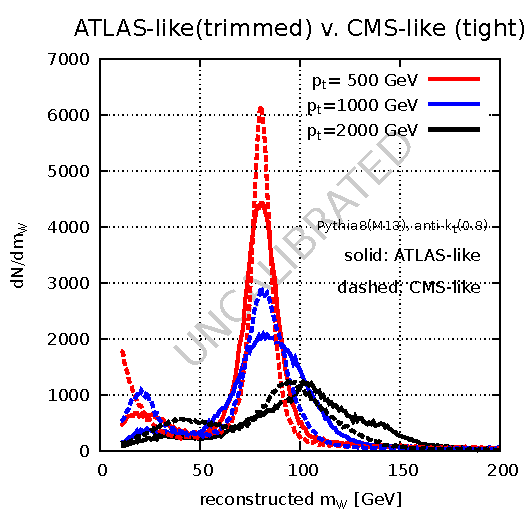
\includegraphics[width=0.45\columnwidth]{jetsub_2prong_mass-detector.pdf}
}
\subfloat[]{
  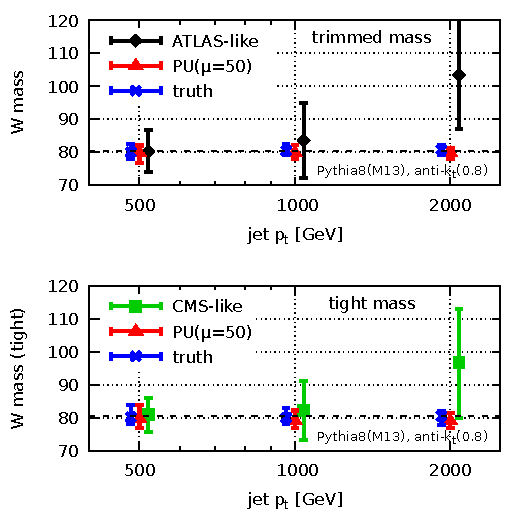
\includegraphics[width=0.45\columnwidth]{jetsub_2prong_mass-width-detector.pdf}
}
  \caption{(a) Mass reconstruction with detector effects at different jet $p_T$.  (b) The peak position and width of the mass distribution, after pileup and, separately, after detector effects.}\label{jetsub_2prong_fig:mass-detector}
\end{figure}

In Fig.~\ref{jetsub_2prong_fig:mass-detector}, we show distributions
of the groomed mass for a hadronically-decaying boosted $W$ boson in
our CMS-like and ATLAS-like detectors at different values of the jet
$p_T$ (Fig.~\ref{jetsub_2prong_fig:mass-detector}a), together with
the measure peak position and width, for the trimmed mass with the
ATLAS-like detector simulation and the tight (mMDT) mass with the
CMS-like simulation (Fig.~\ref{jetsub_2prong_fig:mass-detector}b).%
\footnote{The position and width
  are defined as the median and width of the smallest mass window
  containing 40\% of the events.}
%
We see that the detector has a significant impact on the
distributions: while the $W$ peak remains decent for $500$-GeV jets,
typical of most applications today, the raw resolution considerably
degrades as the $p_T$ is increased.
%
We also see that both detectors show a similar trend, despite their
different approaches.
%
For $p_T$'s up to 1~TeV, it seems that the configuration C gives a
slightly better resolution thans the configuration A, an effect that
is tentatively attributed to particle flow.
%
However, at high $p_T$ there is a trade off between tracking and
calorimetry, which is better in configuration A, leading to comparable detector
resolution.
%
Furthermore, in the full experiments, the reconstruction algorithms
are complementary and adapted to the experiments' detector
technologies, so that the two experiments achieve similar performance.
%
Due to the fact that the end results of the two detectors are quite
similar, we find it unwise to draw any deeper conclusions, since there
are potentially other effects, not included in our simulation, that
could determine the final outcome.
%
We will however point out that, in our (over-simplified) preliminary
studies, the main patterns observed in
Section~\ref{jetsub_2prong_sec:exp_compare}, i.e.\ the overall good
performance of $N_2^{(1,2)}$ and $D_2^{(2)}$ and the interest in
investigating dichroic ratios, seem to remain valid.

Fig.~\ref{jetsub_2prong_fig:mass-detector}b also includes the mass
resolution in the presence of pileup, here Poisson-distributed with an
average multiplicity of 50, mitigated using the SoftKiller method
described in Sec.~\ref{jetsub_2prong_sec:pu_tech}.
%
Based on this simple analysis, it
seems that the reconstruction of $W$ mass peak still behaves properly
in the presence of pileup.
%
It is important to note, however, that this pileup result is in the absence of detector effects, and there is a non-trivial interplay between detector corrections and pileup corrections.

This brief study highlights the essential importance
of understanding detector effects when designing jet substructure
observables.
%
Although we have found that the $N_2$ and $D_2$ observables emphasize,
respectively, performance and robustness, it would also be interesting
to understand if the different detectors played a role in the choice
of one observable as compared with the other.
%
As highlighted by the specific example of the groomed jet mass here, such a study requires considerable care to perform in a meaningful manner.
%
The detectors have a large impact, and the two detectors appear qualitatively similar in our analysis setup.
%
Differences may therefore be due to more subtle features, beyond those included in our study, and this is probably something that is best left to the experimental collaborations to study with realistic detector simulations.
%
We hope that this study motivates the experimental collaborations to further investigate the performance and robustness of different two-prong tagging observables at each of the different steps along the chain of realism in order to understand the different choices in observables.



%%%%%%%%%%%%%%%%%%%%%%%%%%%%%%%%%%%%%%%
\subsection{Polarization Dependence}\label{jetsub_2prong_sec:polar}
%%%%%%%%%%%%%%%%%%%%%%%%%%%%%%%%%%%%%%%

For signal jets, there is another consideration related to the robustness of two-prong tagging, namely the specific nature of the decaying electroweak-scale resonance, which can also affect the substructure observables.
%
Assuming that this electroweak-scale resonance is a color-singlet decaying to quarks, it is completely
characterized by its spin structure.



All of our taggers consist of two conceptually distinct components, which will be affected in different ways by the polarization.
%
We begin by making a cut on the (groomed) mass, followed by a cut on a particular jet shape which is sensitive to the two-prong structure. These two steps are associated with very different physics. A jet from a $W\to q\bar q$ decay consists of two collimated sprays of radiation, which are proxies for the $q$ and $\bar q$, along with radiation emitted from the dipole.
%
Ideally, a groomer should terminate when it de-clusters the jet into two subjets corresponding to the jets initiated by the two quarks.
%
If there is a large fraction of decays where the momentum sharing between the two subjets is hierarchical, though, then the groomer can remove one of the subjets.
%
In this case, the jet will fail the groomed mass criteria.
%
Since the polarization controls the momentum sharing of the subjets, this introduces a sensitivity on the polarization into the tagging procedure.
%
On the other hand, the $2$-prong tagging observables that we consider are all formed as ratios of an observable which is sensitive to radiation from the prongs, divided by a mass-type observable, which (largely) removes the dependence on the momentum sharing of the subjets.

In this subsection, we consider two main issues, namely
the dependence of the standard jet substructure observables to the
polarization of the signals, and the ability to perform polarimetry
using jet substructure observables measured on the hadronic decay
products.

%%%%%%%%%%%%%%%%%%%%%%%%%%%%%%%%%%%%%%%
\subsubsection{Performance Impact of Polarization}\label{jetsub_2prong_sec:polar_robust}
%%%%%%%%%%%%%%%%%%%%%%%%%%%%%%%%%%%%%%%


We begin by studying the sensitivity of two-prong taggers to polarization.
%
To do this, we consider samples of hadronically decaying $W$s, which are either purely transversely polarized, purely longitudinally polarized, or have the Standard Model fraction (mostly transverse).
%
The details of the sample generation were discussed in Sec.~\ref{jetsub_2prong_sec:samples_sub}.


\begin{figure}
\begin{center}
\subfloat[]{\label{jetsub_2prong_fig:polarization_dist}
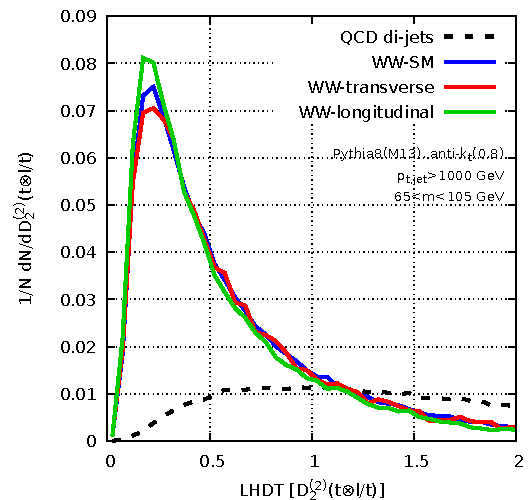
\includegraphics[width=0.4\columnwidth]{jetsub_2prong_D2_polarization}
}
\subfloat[]{\label{jetsub_2prong_fig:polarization_roc}
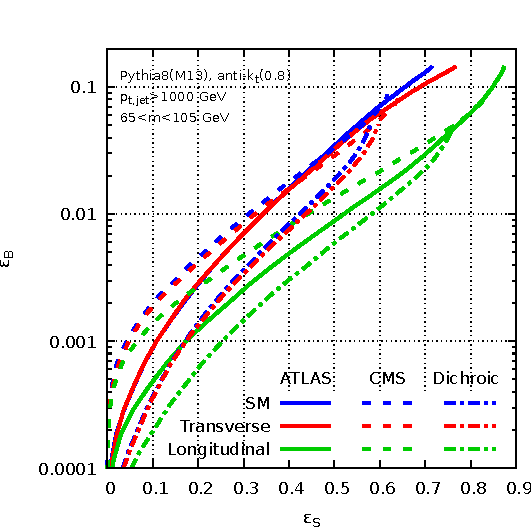
\includegraphics[width=0.4\columnwidth]{jetsub_2prong_polarisation-basic-rocs}
}
\end{center}
\caption{a) Distributions of the $D_2$ observable as measured on the samples with different polarization compositions. These observables are found to be largely insensitive to the polarization. b) ROC curves comparing the different grooming strategies for different polarization samples. While the polarization has a limited effect on the jet shape observables, it modifies the groomed mass acceptance, and therefore the tagging efficiency, significantly.}
\end{figure}


In Fig.~\ref{jetsub_2prong_fig:polarization_dist}, we show the $D_2$ observable as measured on longitudinal and transverse hadronically-decaying W bosons, as well as the Standard Model mixture, as a representative example of the dependence of a two-prong tagger on polarization.
%
From this figure, we see that the jet shape observable itself is remarkably insensitive to the polarization, due to its ratio nature.
%
However, it is important to emphasize that this does not imply that the tagging performance is also independent of the polarization.
%
As can be seen in Fig.~\ref{jetsub_2prong_fig:polarization_roc}, the tagging performance is significantly worse for transversely-polarized $W$ bosons as compared with longitudinally-polarized $W$ bosons.
%
This is due to the fact that transversely-polarized $W$ bosons have a more asymmetric energy sharing, and it is therefore more likely that one of the subjet prongs is groomed away, leading to the jet failing the mass cut.
%
This difference between longitudinally and transversely-polarized bosons should be taken into account in studies at the LHC.
%
It would also be interesting to develop tagging or reconstruction schemes that are less sensitive to polarization.




%%%%%%%%%%%%%%%%%%%%%%%%%%%%%%%%%%%%%%%
\subsubsection{Tagging Longitudinal vs.\ Transverse Bosons}\label{jetsub_2prong_sec:polar_tag}
%%%%%%%%%%%%%%%%%%%%%%%%%%%%%%%%%%%%%%%

Having understood the dependence of standard jet substructure observables on polarization, it is interesting to know whether jet substructure observables are able to tag distinct polarizations on hadronically-decaying particles, and with what efficiency this can be done.
%
Here, we do not perform a comprehensive study, but restrict ourselves to studying a particular example of an observable which is sensitive to the $W$ polarization, and we evaluate its performance for distinguishing transverse and longitudinal $W$ bosons. 

The sole impact of the polarization of the decaying object is to determine the kinematics of the decaying subjets.
%
Indeed, this can be made rigorous in the sense of a factorization theorem for boosted jets in the two-prong limit.
%
We are therefore interested in an observable that is sensitive to the kinematics of the two subjets.
%
While a variety of different observables could be considered, here we consider the $z_g$ observable \cite{Larkoski:2014wba,Larkoski:2014bia,Larkoski:2015lea}, which measures the momentum sharing of the subjets. The precise definition of $z_g$ was given in Sec.~\ref{jetsub_2prong_sec:groom_tech}, which we recall for convenience
\begin{align}
z_g=\frac{\min\left[ p_{Ti}, p_{Tj}  \right]}{p_{Ti}+p_{Tj}}\,.
\end{align}
Here $p_{Ti}$ and $p_{Tj}$ are the momenta of the first set of subjets that pass the SoftDrop criteria.


Since we are focused on robustness in this paper, it is also worth commenting on the robustness of the $z_g$ observable. For signal jets, since this observable measures global energy properties of the subjets, it is stable.
%
Interestingly, it is also remarkably stable on the background, where it flows in the high-$p_T$ limit to the QCD splitting function \cite{Larkoski:2015lea}.

In Fig.~\ref{jetsub_2prong_fig:z_g_dist}, we show the $z_g$ distribution for different polarized $W$ bosons.
%
For reference, the $z_g$ distribution for QCD dijets is also shown.
%
The $z_g$ distribution for transversely-polarized $W$ bosons follows most closely the QCD distribution, as expected, being peaked at small values of $z_g$.
%
On the other hand, for longitudinally-polarized $W$ bosons, the $z_g$ distribution is peaked at high values of $z_g$.
%
This illustrates that the $z_g$ observable is indeed behaving as expected, and is achieving sensitivity to the polarization of the decaying $W$ boson only from its hadronic decay products.
%
In Fig.~\ref{jetsub_2prong_fig:z_g_roc}, we show  the ROC curve for separating longitudinal from transverse $W$ bosons.
%
Here we see that $z_g$ provides moderate separation power for tagging the polarization of the decaying $W$ bosons.
%
It would be interesting to investigate this further to see if more ideal observables could be found, however, we are not optimistic that significant improvement can be achieved, since the primary imprint of the polarization should be in the kinematics of the subjets.

\begin{figure}
\begin{center}
\subfloat[]{\label{jetsub_2prong_fig:z_g_dist}
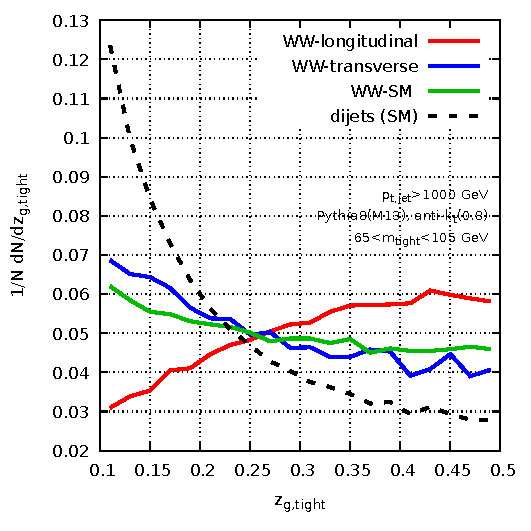
\includegraphics[width=0.45\columnwidth]{jetsub_2prong_polarisation-zg-distrib}
}
\subfloat[]{\label{jetsub_2prong_fig:z_g_roc}
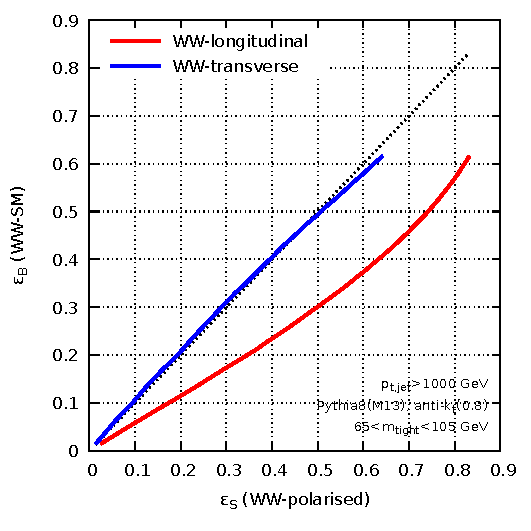
\includegraphics[width=0.45\columnwidth]{jetsub_2prong_polarisation-zg-roc}
}
\end{center}
\caption{a) The $z_g$ distribution as measured on boosted $W$ samples with different polarization compositions. Transversely-polarized $W$s behave similarly to the QCD background, while decent separation is observed between longitudinally- and transversely-polarized $W$s. b) A ROC curve showing the separation between transversely- and longitudinally-polarized $W$ bosons using the $z_g$ observable. Moderate separation is observed.}
\end{figure}



%%%%%%%%%%%%%%%%%%%%%%%%%%%%%%%%%%%%%%%
\subsection{Summary and Recommendations}\label{jetsub_2prong_sec:conc}
%%%%%%%%%%%%%%%%%%%%%%%%%%%%%%%%%%%%%%%

In this paper, we performed a comprehensive study of performance and robustness for two-prong tagging, and provided a unifying approach to understanding different classes of two-prong taggers based on dichroic observables, which allow for different amounts of grooming in the numerator and denominator of observables.
%
We introduced measures of robustness, in addition to the standard measures of performance, and we used these measures to study the robustness of two-prong taggers to theory issues, namely hadronization and underlying event.
%
We believe that these will be of more general utility in jet substructure, and could be applied also to study three-prong tagging, for example.

As a part of our study, we have also introduced a number of new dichroic observables, which generalize the dichroic $N$-subjettiness observables to observables formed from the energy correlation functions.
%
This offers a general and unifying approach to designing new jet substructure observables which are simultaneously performant and resilient.
%
We have shown that the $N_2$-style observables used by CMS tend to be more performant, but less resilient than the $D_2$-style observables used by ATLAS.
%
For a given observable, we have found that moving to a dichroic variant can typically improve performance without significantly decreasing its robustness to hadronization.

We have also studied the effect of polarization on two-prong taggers.
%
We found that while polarization has minimal effect on standard two-prong tagging observables, since they are typically defined as ratios, it has a large effect on their tagging efficiency due to applied mass cuts.
%
Significantly better tagging performance is observed for longitudinally-polarized bosons.
%
An interesting avenue beyond standard two-prong tagging is using jet substructure observables to tag the polarization of decaying Standard Model bosons using their hadronic decay products.
%
We proposed the observable $z_g$, which measures the momentum sharing asymmetry between subjets, as an effective polarization tagger.
%
We illustrated that separation between longitudinal and transverse bosons can be achieved.
%
It would be interesting to study this problem in more detail.

We have identified a  number of new two-prong taggers that outperform, in both robustness and tagging performance, those currently used by the ATLAS and CMS collaborations.
%
These findings are summarized in Fig.~\ref{jetsub_2prong_fig:phasespace}, which also lists a number of promising new observables.
%
We therefore believe that further studies using more detailed simulations of the ATLAS and CMS detectors, and ultimately on real data, would be of significant interest.
%
More generally, we expect that the emphasis on a simultaneous evaluation of the performance and robustness, as well as the particular metrics introduced in this paper, will play a significant role in future studies of jet substructure techniques at the LHC.

%%%%%%%%%%%%%%%%%%%%%%%%%%%%%%%%%%%%%%%
\subsection*{Acknowledgments}
%%%%%%%%%%%%%%%%%%%%%%%%%%%%%%%%%%%%%%%

We thank the participants of Les Houches 2017 for a lively environment and useful discussions.
%
The work of GS is supported in part by the Paris-Saclay IDEX under the
IDEOPTIMALJE grant, by the French Agence Nationale de la Recherche,
under grant ANR-15-CE31-0016, and by the ERC Advanced Grant Higgs@LHC
(No.\ 321133).
%
The work of JT is supported by the DOE under grant contract numbers DE-SC-00012567 and DE-SC-00015476.
%
The work of IM is supported by Office of High Energy Physics of the U.S. Department of Energy under Contract No. DE-AC02-05CH11231, and the LDRD Program of LBNL.


%%%%%%%%%%%%%%%%%%%%%%%%%%%%%%%%%%%%%%%
%\end{acknowledgments}
%%%%%%%%%%%%%%%%%%%%%%%%%%%%%%%%%%%%%%%



\bibliography{lh2017_2prong}

\end{document}
